\documentclass{scrartcl}
\usepackage{pgfplots}\usepackage{cancel}
\usepackage{booktabs} % For better table formatting
\usepackage{calc}
\usepackage{Style_File}
\newcommand{\ad}[1]{a_{#1}^\dagger}
\usepackage{fancyhdr}
\usepackage{tensor}
\usepackage{array}
\usepackage{lmodern}
\definecolor{violet}{rgb}{0.5,0.27,0.45}
\tikzstyle{tensor}=[rectangle,draw=blue!50,fill=blue!20,thick]

\newcolumntype{P}[1]{>{\centering\arraybackslash}p{#1}}
% Recommended preamble:
\usetikzlibrary{arrows.meta}
\usetikzlibrary{backgrounds}
\usepgfplotslibrary{patchplots}
\usepgfplotslibrary{fillbetween}
\pgfplotsset{%
    layers/standard/.define layer set={%
        background,axis background,axis grid,axis ticks,axis lines,axis tick labels,pre main,main,axis descriptions,axis foreground%
    }{
        grid style={/pgfplots/on layer=axis grid},%
        tick style={/pgfplots/on layer=axis ticks},%
        axis line style={/pgfplots/on layer=axis lines},%
        label style={/pgfplots/on layer=axis descriptions},%
        legend style={/pgfplots/on layer=axis descriptions},%
        title style={/pgfplots/on layer=axis descriptions},%
        colorbar style={/pgfplots/on layer=axis descriptions},%
        ticklabel style={/pgfplots/on layer=axis tick labels},%
        axis background@ style={/pgfplots/on layer=axis background},%
        3d box foreground style={/pgfplots/on layer=axis foreground},%
    },
}
\newcommand{\amstitle}[1]{%
  {\Large\MakeUppercase{#1}}% First letter large, rest small caps (simplified)
  % OR for true small caps:
  % {\Large\MakeUppercase{\expandafter\@firstofone#1}\scshape\MakeLowercase{#1}}%
}
\usepackage[left = 1in,
right = 1in,
bottom = 1.4in,
top = 1in,
a4paper]{geometry}


\fancyhead[L,C]{}
\fancyhead[R]{Notes}
\usepackage[hidelinks]{hyperref}
\hypersetup{colorlinks=true,linkcolor=cyan!80!black, citecolor=YellowOrange,urlcolor=cyan!80!black}
\fancyhead[L]{ Tensor Calculus}
\fancyfoot[C]{\thepage}
\fancyfoot[R,L]{}
\usetikzlibrary{calc}
\pagestyle{fancy}
\renewcommand{\headrulewidth}{0.4pt}
\definecolor{titleblue}{RGB}{0, 80, 120}
\usepackage{longtable} 


\begin{document}
\makeatletter
\begin{titlepage}
    \begin{tikzpicture}[remember picture, overlay]
        \draw[black!80!blue, line width=2pt] 
            ($(current page.north west)+(0.6cm,-0.6cm)$) rectangle 
            ($(current page.south east)+(-0.6cm,0.6cm)$);
    \end{tikzpicture}
    \vspace*{2cm}
    
        \begin{center}
            {\rmfamily
                \Huge{\textcolor{blue!30!black}{%
                    \textmd{{\HUGE{{T}}}}ensor {\HUGE C}alculus
                }}\\[0.7cm]
               
                
                \Large \textsc{Notes} \\[0.3cm]
               \Large \textit{Based on: many different sources}\\[0.5cm]

            }
            \end{center}
      \begin{figure}[H]
        \centering 
         


\tikzstyle{tensor}=[rectangle,draw=blue!50,fill=blue!20,thick]

\begin{tikzpicture}[scale=1.5, inner sep=1mm]
    \foreach \i in {1,...,5} {
        \node[tensor] (\i) at (\i, 0) {};
        \node (\i spin) at (\i, -0.7) {};
        \draw[-] (\i) -- (\i spin);
    };
    \foreach \i in {1,...,4} {
        \pgfmathtruncatemacro{\iplusone}{\i + 1};
        \draw[-] (\i) -- (\iplusone);
    };
    \draw[-] (1.west) .. controls +(-1.5, 1) and +(1.5, 1) .. (5.east);
\end{tikzpicture}

      \end{figure}
       
        \vspace{1cm}
        \begin{center}
           \Large \texttt{\textbf{{\LARGE  S}agnik {\LARGE S}eth }}
        \end{center}
        \vspace{0.5cm}
      \begin{center}
    \textbf{ Dept of Physical Sciences} \\
    \textbf{IISER Kolkata}
    \vspace{0.5cm}

    % Side-by-side logos
   
\end{center}

\end{titlepage}

  
       
\tableofcontents
\newpage
\section{Introduction}
Hehe......\emoji{sweat-smile} I am writing this as a way to understand tensors better and also to do something ``productive''. I don't know how much I will be able to complete but I intend to touch upon the basic aspects, albeit, in an extremely non-rigorous way....not going into heavy math (which I think is very bad 'coz math is great \emoji{winking-face}). I will try to do some proofs (which I feel like doing) and skip others (since I don't care). I will definitely take $c=1$ unless its necessary not to. I will use the convention $(+,-,-,-)$ for the metric tensor. I will also use some gen alpha slangs (which will indicate how chill I am!) and overall try to write in a fun way. A few references which I will use are listed below:
\begin{itemize}
    \item \textit{Tensor Calculus for Physics: A Concise Guide
} by Dwight E Neuenschwander
\item \textit{The Poor Man’s Introduction to Tensors} by Justin C. Feng
\item \textit{Geometry, Topology and Physics} by Mikio Nakahara
\item Tensor Calculus YouTube video series by eigenchris and Andrew Dotson
\end{itemize}
I will continue to add the resources as I progress. I am writing this as my own personal notes and if it helps anyone else, I will be super happy. If any mistake is there, let me know! \emoji{victory-hand}
\section{Indices: the ultimate rizzler!}
Indices make our lives easier when writing abstract quantitites having multiple components, like vectors. If we have a three-dimensional vector, we can write it as $v\indices{^i}$ where $i$ can take the values $1$, $2$, or $3$.\\[0.3cm]
 Why are the indices written as superscript? Well, these are contravariant indices which will be discussed later. For now, let's just say that `upstairs' indices are the `normal thing'. Index placement is important and these are not powers...just the way we denote the components.\\[0.3cm]
 Consider the (in)famous equation: 
 $$\mathbf{F}= m \mathbf{a}$$
 This can be written as $F\indices{^i} = m a\indices{^i}$, for each component $i$. Just remember that we should have the same kind of indices on both side of the equation finally. That is, if we have `upstairs' index on the right, same should be on the left.\\[0.3cm]
 \subsection{Einstein Convention}
 The OG rule...whenever you see two same indices, sum them.  That's it! Let's make our hands dirty and look at some examples:\\[0.3cm]
 \subsection{Examples}
 \textbf{Matrix Multiplication:}\\[0.3cm]
 Let us have the eigenvalue equation $M\mathbf{v} = \lambda\mathbf{v}$. We can write this as: 
 $$\sum\limits_j M_{ij}v^j = \lambda v^i$$
 Note two things here: 
 \begin{itemize}
    \item The index $j$ is summed over, so it does not come in the final expression (dummy index!).
    \item The index $i$ occurs as a superscript on the right, so in the left also, the final expression should have the index $i$ as a superscript.
 \end{itemize}
 Thus, using Einstein convention and correct index placement, the above equation can be written as:
$$M\indices*{^i_j}v\indices{^j} = \lambda v\indices{^i}$$
This can be visualised by treating each quantity as a `box' with the indices as some `hands' protruding out. When we sum, we just join these `hands'. After taking the sum, the number of free hands decreases (index contraction)l A matrix has two hands and a vector has one hand. When we multiply a matrix with a vector, we obtain a vector, which should have one hand. This is represented in the diagram below:
\begin{figure}[H]
    \centering
    

\tikzset{every picture/.style={line width=0.75pt}} %set default line width to 0.75pt        

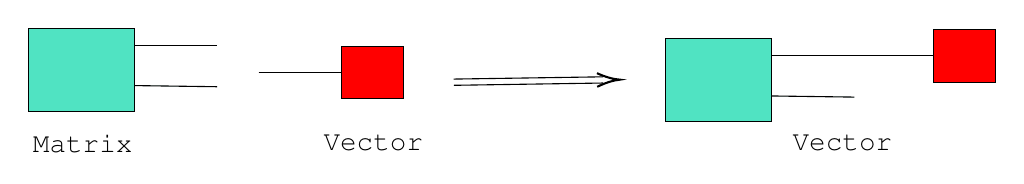
\begin{tikzpicture}[x=0.75pt,y=0.75pt,yscale=-1,xscale=1]
%uncomment if require: \path (0,300); %set diagram left start at 0, and has height of 300

%Shape: Rectangle [id:dp9056942194735556] 
\draw  [fill={rgb, 255:red, 80; green, 227; blue, 194 }  ,fill opacity=1 ] (100,112) -- (151,112) -- (151,152) -- (100,152) -- cycle ;
%Straight Lines [id:da9172659624339214] 
\draw [fill={rgb, 255:red, 80; green, 227; blue, 194 }  ,fill opacity=1 ]   (151,120.18) -- (191,120.18) ;
%Straight Lines [id:da2833939201314972] 
\draw [fill={rgb, 255:red, 80; green, 227; blue, 194 }  ,fill opacity=1 ]   (151,139.63) -- (191,140.18) ;

%Shape: Rectangle [id:dp6422275710126122] 
\draw  [fill={rgb, 255:red, 255; green, 0; blue, 0 }  ,fill opacity=1 ] (251,120.63) -- (281,120.63) -- (281,146) -- (251,146) -- cycle ;
%Straight Lines [id:da9091154996581836] 
\draw [fill={rgb, 255:red, 255; green, 0; blue, 0 }  ,fill opacity=1 ]   (211,133.18) -- (251,133.18) ;

%Straight Lines [id:da6668729559343063] 
\draw    (304.98,136.5) -- (376.98,135.41)(305.02,139.5) -- (377.02,138.4) ;
\draw [shift={(385,136.78)}, rotate = 179.13] [color={rgb, 255:red, 0; green, 0; blue, 0 }  ][line width=0.75]    (10.93,-3.29) .. controls (6.95,-1.4) and (3.31,-0.3) .. (0,0) .. controls (3.31,0.3) and (6.95,1.4) .. (10.93,3.29)   ;
%Shape: Rectangle [id:dp5499160435625281] 
\draw  [fill={rgb, 255:red, 80; green, 227; blue, 194 }  ,fill opacity=1 ] (407,117) -- (458,117) -- (458,157) -- (407,157) -- cycle ;
%Straight Lines [id:da11942666503370314] 
\draw [fill={rgb, 255:red, 80; green, 227; blue, 194 }  ,fill opacity=1 ]   (458,125.18) -- (498,125.18) ;
%Straight Lines [id:da4684372747610551] 
\draw [fill={rgb, 255:red, 80; green, 227; blue, 194 }  ,fill opacity=1 ]   (458,144.63) -- (498,145.18) ;

%Shape: Rectangle [id:dp9126568397813256] 
\draw  [fill={rgb, 255:red, 255; green, 0; blue, 0 }  ,fill opacity=1 ] (536,112.63) -- (566,112.63) -- (566,138) -- (536,138) -- cycle ;
%Straight Lines [id:da5617556659509985] 
\draw [fill={rgb, 255:red, 255; green, 0; blue, 0 }  ,fill opacity=1 ]   (496,125.18) -- (536,125.18) ;


% Text Node
\draw (101,162) node [anchor=north west][inner sep=0.75pt]   [align=left] {{\fontfamily{pcr}\selectfont Matrix}};
% Text Node
\draw (241,162) node [anchor=north west][inner sep=0.75pt]   [align=left] {{\fontfamily{pcr}\selectfont Vector}};
% Text Node
\draw (467,162) node [anchor=north west][inner sep=0.75pt]   [align=left] {{\fontfamily{pcr}\selectfont Vector}};


\end{tikzpicture}

    \caption{Matrix-vector multiplication. The final product has one free hand and is thus a vector.}
\end{figure}
\noindent
\textbf{The Scalar Product:}\\[0.3cm]
The dot product or scalar product of two vectors is a scalar (no hand). Then, there should be no free index in the expression. Thus, in the index notation:
$$\mathbf{v}\cdot \mathbf{v} = v\indices{^i}v\indices{_i} =v\indices{_i}v\indices{^i}  $$
The last two expressions are same. The upstairs or downstairs indices do not matter, as these are summed over. Note that in this definition, we have used a \textit{dual vector}, having a lower index. We can also define the dot product using the \textit{regular} vector with an upper index but then a \textit{metric} comes in.
\begin{figure}[H]
    \centering
    

\tikzset{every picture/.style={line width=0.75pt}} %set default line width to 0.75pt        

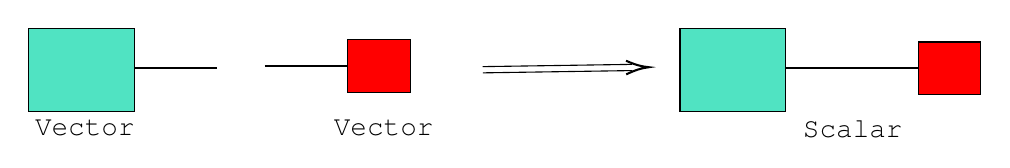
\begin{tikzpicture}[x=0.75pt,y=0.75pt,yscale=-1,xscale=1]
%uncomment if require: \path (0,300); %set diagram left start at 0, and has height of 300

%Shape: Rectangle [id:dp5798300081474196] 
\draw  [fill={rgb, 255:red, 80; green, 227; blue, 194 }  ,fill opacity=1 ] (100,112) -- (151,112) -- (151,152) -- (100,152) -- cycle ;
%Straight Lines [id:da22962560201461135] 
\draw [fill={rgb, 255:red, 80; green, 227; blue, 194 }  ,fill opacity=1 ]   (151,131.18) -- (191,131.18) ;
%Shape: Rectangle [id:dp20432070859726514] 
\draw  [fill={rgb, 255:red, 255; green, 0; blue, 0 }  ,fill opacity=1 ] (254,117.63) -- (284,117.63) -- (284,143) -- (254,143) -- cycle ;
%Straight Lines [id:da524122200138993] 
\draw [fill={rgb, 255:red, 255; green, 0; blue, 0 }  ,fill opacity=1 ]   (214,130.18) -- (254,130.18) ;

%Straight Lines [id:da7051909181445478] 
\draw    (318.98,130.5) -- (390.98,129.41)(319.02,133.5) -- (391.02,132.4) ;
\draw [shift={(399,130.78)}, rotate = 179.13] [color={rgb, 255:red, 0; green, 0; blue, 0 }  ][line width=0.75]    (10.93,-3.29) .. controls (6.95,-1.4) and (3.31,-0.3) .. (0,0) .. controls (3.31,0.3) and (6.95,1.4) .. (10.93,3.29)   ;
%Shape: Rectangle [id:dp6270655055347218] 
\draw  [fill={rgb, 255:red, 80; green, 227; blue, 194 }  ,fill opacity=1 ] (414,112) -- (465,112) -- (465,152) -- (414,152) -- cycle ;
%Straight Lines [id:da6216765005210074] 
\draw [fill={rgb, 255:red, 80; green, 227; blue, 194 }  ,fill opacity=1 ]   (465,131.18) -- (505,131.18) ;
%Shape: Rectangle [id:dp601921472040452] 
\draw  [fill={rgb, 255:red, 255; green, 0; blue, 0 }  ,fill opacity=1 ] (529,118.63) -- (559,118.63) -- (559,144) -- (529,144) -- cycle ;
%Straight Lines [id:da020089358658374357] 
\draw [fill={rgb, 255:red, 255; green, 0; blue, 0 }  ,fill opacity=1 ]   (489,131.18) -- (529,131.18) ;


% Text Node
\draw (102,155) node [anchor=north west][inner sep=0.75pt]   [align=left] {{\fontfamily{pcr}\selectfont Vector}};
% Text Node
\draw (246,155) node [anchor=north west][inner sep=0.75pt]   [align=left] {{\fontfamily{pcr}\selectfont Vector}};
% Text Node
\draw (472,155) node [anchor=north west][inner sep=0.75pt]   [align=left] {{\fontfamily{pcr}\selectfont Scalar}};


\end{tikzpicture}

    \caption{Dot product of two vectors. The final product is a scalar and has no free hands.}
\end{figure}
\noindent
So basically a \textit{scalar} is something that does not change under coordinate transformation, that is, if we go from a coordinate $(x,y,z)$ to $(x',y',z')$, a scale $\lambda = \lambda'$.\\[0.3cm]
\textbf{Euclidean Vectors:}\\[0.3cm]
Any vector can be written as in terms of basis vectors: $\mathbf{A} = \tensor{A}{^i}\mathbf{e}_i$ where $A^i$ are the components of the vector in the chosen basis. Now, we define $$\mathbf{e}_n\cdot \mathbf{e}_m = g_{nm}$$
These $g_{nm}$ are coefficients of metric tensor which will be discussed later. If these basis vectors are orthonormal, then the coefficients become the kronecker delta. Then we have the scalar product:
\begin{align*}
    \mathbf{A}\cdot \mathbf{B} &=  (\tensor{A}{^m}\mathbf{e}_m)\cdot  \tensor{B}{^n}\mathbf{e}_n\\
    &=(\tensor{A}{^m}\tensor{B}{^n}\mathbf{e}_m)\cdot  \mathbf{e}_n\\
    &=\tensor{A}{^m}\tensor{B}{^n}g_{nm}
\end{align*}
Note that we have used the \textit{regular vector} with an upper index here, with the metric $g$. We can define a cross product of two vectors as:
$$(\mathbf{A}\times \mathbf{B})^i = \epsilon^{ijk}A^jB^k$$
where $\epsilon^{ijk}$ is the Levi-Civita symbol (cyclic permutation of ${i,j,k}$ gives 1 and non-cyclic permutation gives -1 while repeated index in the symbol gives 0). \\[0.3cm]
\subsection{Some vector BS}
\textbf{Vectors as Directional Derivatives:}\\[0.3cm]
A vector can be thought of as a directional derivative. We define the directional derivative operator as:
$$\mathbf{v}\cdot \nabla = v^i \partial_i\equiv  v^i \dfrac{\partial}{\partial x^i}$$
This is very similar to the vector expansion in terms of the basis vectors. Thus, the partial derivatives somewhat act like a basis. The basis of partial derivatives is indeed called a \textit{coordinate basis}. Now let us calculate:
$$\mathbf{v}\cdot \nabla x^j = v^i \partial_i x^j = v^i\pdv{x^j}{x^i} = v^i\tensor*{\delta}{^j_i} = v^j$$
We have used the fact that coordinate components are independent of each other, that is, partial derivative of one component with respect to another gives a kronecker delta. Note that we have used the proper index placement here: $\partial_j\equiv \pdv{x^j}$ has a lower index (by definition) while $x^j$ has an upper index, thus kronecker delta has an upper as well as lower index.\\[0.3cm]
Now, let us consider we have a position vector written in a basis $\{\veb{e}_i\}$, that is, $$\veb{r} = x^i \veb{e}_i$$
Since $\veb{r}$ depends on the coordinate $\{x^i\}$, we can expand the differential displacement as:
\begin{align*}
    d\veb{r} &= \pdv{\veb{r}}{{x}^i}dx^i \\
    &= \pdv{(x^j \veb{e}_j)}{x^i}dx^i \\
    &=\brac{\pdv{x^j }{x^i}\veb{e}_j + \pdv{ \veb{e}_j}{x^i}x^j }dx^i
\end{align*}
The second term is zero as the basis vectors are independent of the coordinates and the first term gives Kronecker delta, thus we have:
$$d\veb{r} = \veb{e_i}dx^i $$
Comparing this with the first line of the previous expansion we have:
$$\boxed{\veb{e}_i = \pdv{\veb{r}}{x^i}}$$
Thus any basis vector can be obtained from the partial derivative of the position vector with respect to the coordinates.\\[0.3cm] 
\textbf{Vector Transformation:}\\[0.3cm]
Let us suppose we have a coordinate system $(x,y,z)$ and we rotate it about the $z$-axis by an angle $\theta$. The new coordinates are given by:
\begin{figure}[H]
    \centering 
    

\tikzset{every picture/.style={line width=0.75pt}} %set default line width to 0.75pt        

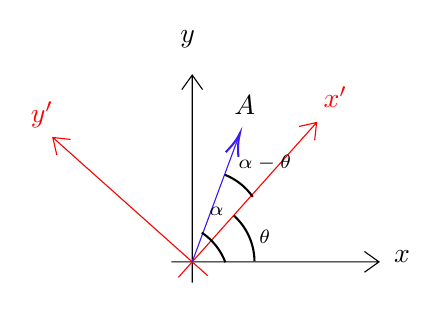
\begin{tikzpicture}[x=0.75pt,y=0.75pt,yscale=-1,xscale=1]
%uncomment if require: \path (0,201); %set diagram left start at 0, and has height of 201

%Shape: Axis 2D [id:dp5999262441064296] 
\draw  (283,150) -- (383,150)(293,60) -- (293,160) (376,145) -- (383,150) -- (376,155) (288,67) -- (293,60) -- (298,67)  ;
%Shape: Axis 2D [id:dp6999025250833045] 
\draw [color={rgb, 255:red, 255; green, 0; blue, 0 }  ,draw opacity=1 ] (286.34,157.46) -- (352.93,82.85)(225.85,90.07) -- (300.46,156.66) (344.54,84.75) -- (352.93,82.85) -- (352,91.41) (227.75,98.46) -- (225.85,90.07) -- (234.41,91)  ;
%Shape: Arc [id:dp9879953663640971] 
\draw  [draw opacity=0][line width=0.75]  (313.11,127.73) .. controls (319.05,133.11) and (322.85,140.84) .. (323,149.49) .. controls (323,149.54) and (323,149.6) .. (323,149.65) -- (293,150) -- cycle ; \draw  [line width=0.75]  (313.11,127.73) .. controls (319.05,133.11) and (322.85,140.84) .. (323,149.49) .. controls (323,149.54) and (323,149.6) .. (323,149.65) ;  
%Straight Lines [id:da08151702925178561] 
\draw [color={rgb, 255:red, 59; green, 27; blue, 243 }  ,draw opacity=1 ]   (293,150) -- (315.3,89.91) ;
\draw [shift={(316,88.03)}, rotate = 110.36] [color={rgb, 255:red, 59; green, 27; blue, 243 }  ,draw opacity=1 ][line width=0.75]    (10.93,-3.29) .. controls (6.95,-1.4) and (3.31,-0.3) .. (0,0) .. controls (3.31,0.3) and (6.95,1.4) .. (10.93,3.29)   ;
%Shape: Arc [id:dp7996887661941752] 
\draw  [draw opacity=0][line width=0.75]  (297.62,135.89) .. controls (302.69,139.3) and (306.73,144.24) .. (308.98,150.2) -- (280.91,160.81) -- cycle ; \draw  [line width=0.75]  (297.62,135.89) .. controls (302.69,139.3) and (306.73,144.24) .. (308.98,150.2) ;  
%Shape: Arc [id:dp8674168141053495] 
\draw  [draw opacity=0][line width=0.75]  (308.79,108.05) .. controls (314.04,110.15) and (318.74,113.75) .. (322.19,118.68) -- (297.62,135.89) -- cycle ; \draw  [line width=0.75]  (308.79,108.05) .. controls (314.04,110.15) and (318.74,113.75) .. (322.19,118.68) ;  

% Text Node
\draw (324,133.4) node [anchor=north west][inner sep=0.75pt]  [font=\scriptsize]  {$\theta $};
% Text Node
\draw (389,143.43) node [anchor=north west][inner sep=0.75pt]    {$x$};
% Text Node
\draw (286,37.43) node [anchor=north west][inner sep=0.75pt]    {$y$};
% Text Node
\draw (355,64.43) node [anchor=north west][inner sep=0.75pt]  [color={rgb, 255:red, 255; green, 0; blue, 0 }  ,opacity=1 ]  {$x'$};
% Text Node
\draw (214,71.43) node [anchor=north west][inner sep=0.75pt]  [color={rgb, 255:red, 255; green, 0; blue, 0 }  ,opacity=1 ]  {$y'$};
% Text Node
\draw (300,122.4) node [anchor=north west][inner sep=0.75pt]  [font=\scriptsize]  {$\alpha $};
% Text Node
\draw (312,68.43) node [anchor=north west][inner sep=0.75pt]    {$A$};
% Text Node
\draw (314,97.4) node [anchor=north west][inner sep=0.75pt]  [font=\scriptsize]  {$\alpha -\theta $};


\end{tikzpicture}
l
\end{figure}
$$x' = x\cos\theta - y\sin\theta$$
$$y' = x\sin\theta + y\cos\theta$$
$$z' = z$$
These relations can be readily found out using the following: Suppose we have a point $A$ making an angle $\alpha$ with the original system. Then we have $x = r\cos(\alpha), y = r\sin(\alpha)$. After rotation, the new coordinates are given by:
$$x' = r\cos(\alpha - \theta) = r\cos\alpha\cos\theta + r\sin\alpha\sin\theta$$
$$y' = r\sin(\alpha - \theta) = r\sin\alpha\cos\theta - r\cos\alpha\sin\theta$$
which gives the previous result. Note that the $z$ coordinate does not change as the rotation is about the $z$-axis. Now we consider the infinitesimal displacement in the new coordinate frame:
\begin{align*}
    (ds')^2 &= (dx')^2 + (dy')^2 + (dz')^2\\
    &= (dx\cos\theta - dy\sin\theta)^2 + (dx\sin\theta + dy\cos\theta)^2 + dz^2\\
    &= dx^2(\cos^2\theta+\sin^2\theta) + dy^2(\cos^2\theta+\sin^2\theta)- \cancel{2dxdy\sin\theta\cos\theta} +  \cancel{2dxdy\sin\theta\cos\theta} + dz^2\\
    &= dx^2 + dy^2 + dz^2\\
    &= ds^2
\end{align*}
Thus we see that the infinitesimal displacement is invariant under coordinate transformation and is thus a scalar.\\[0.3cm]
Now, note one thing: If we consider the new coordinates as a function of the old coordinate that is $x' \equiv x'(x,y,z)$, we can write: 
$$(dx')^i = \pdv{x'^i}{x^j}dx^j$$
Using this analogy, we can define the transformation of a vector as:
$$(v')^i = \pdv{x'^i}{x^j}v^j$$
Thus a vector is a quantity which transform like this. The terms $\pdv{x'^i}{x^j}$ are the components of the transformation matrix $\tensor*{\Lambda}{^i_j}$.
As we defined the transformation from $x$ to $x'$, we can also define the reverse transformation from $x'$ to $x$ as:
\begin{align*}
    x^i &= \pdv{x^i}{x'^j} x'^j \\
    & =  \brac{\pdv{x^i}{x'^j}\pdv{x'^j}{x^k}}x^k \\
\end{align*}
Now in the above sum, $j$ and $k$ indices are summed over. We must obtain $x^i$ from the right hand side also. Thus by observation, we can see that the term $\pdv{x^i}{x'^j}\pdv{x'^j}{x^k}$ must be equal to the kronecker delta $\tensor*{\delta}{^i_k}$.

\section{Contravariant and Covariant: why the skibidi!}
Let us suppose we have a vector space $\mathbf{V}$ and two bases $\{\mathbf{e}_i\}$ and $\{\mathbf{e}'_i\}$. We can the write the transformation of the basis into one another as:
\begin{align*}
    \mathbf{e}_i &= \tensor*{\Lambda}{^j_i}\mathbf{e}'_j\\
    \mathbf{e}'_i &= \tensor*{(\Lambda^{-1})}{_i^j}\mathbf{e}_j
\end{align*}
Now if we have a vector, we can write it in terms of the basis vectors as:
$$\mathbf{x} =  (x')^j \mathbf{e}'_j = x^i \mathbf{e}_i = (x^i \tensor*{\Lambda}{^j_i}) \mathbf{e}'_j $$
From this we get: $(x')^j = \tensor*{\Lambda}{^j_i} x^i$. Well note that, in the transformation equation of the basis, if we have the primed basis in the left, then we had the inverse transformation matrix $\Lambda^{-1}$ in the right, but here it is different (primed component in the left and $\Lambda$ in the right). Thus, the basis vectors and the components transform in the ``opposite'' or ``\textbf{contra}ry'' way. Thus, these components are called the \textbf{contravariant} components of the vector.\\[0.3cm]
Let us now consider the dual space $\mathbf{V}^*$\footnote{The dual space is the set of all linear functionals, that is, linear maps $f: \mathbf{V} \to \mathbb{R}$.} of the vector space $\mathbf{V}$. From the linearity property, we have:
$$f(x^i\mathbf{e}_i) = x^i f(\mathbf{e}_i) \equiv x^i f_i$$
Now, we use the basis transformation equation:
$$f_i = f(\mathbf{e}_i) = f(\tensor*{\Lambda}{^j_i}\mathbf{e}'_j) = \tensor*{\Lambda}{^j_i}f(\mathbf{e}'_j) = \tensor*{\Lambda}{^j_i}f'_j$$
These $f_i$ are the components of the ``dual vector''. Note that if we have unprimed things on the left, then we have the transformation matrix $\Lambda$ on the right, which is similar to the transformation of the basis. Thus, we see that this transformation follows the same transformation as the basis vectors. Thus, these components are called the \textbf{covariant} components of the vector.\\[0.3cm]
So, the components are named according to how the basis vectors transform. If they transform together, the are called \textbf{co}variant (and denoted by downstairs index) and if they transform in the opposite way, they are called \textbf{contra}variant (and denoted by upstairs index). The contravariant and the covariant components together form an `invariance' like the scalar product (which do not change under coordinate transformation):
$$\veb{v}\cdot\veb{v} = v_i v^i $$
\noindent
We had earlier seen another definition of the inner product, using both contravariant components and the matric tensor, which was $\veb{v}\cdot\veb{v} = v^i v^j g_{ij}$. Comparing both these definitions, we can see a relation:
$$v_i = g_{ij} v^j$$
Thus when changing from contravariant to covariant, we just need to invoke the holy metric tensor (to be dicussed later further).\\[0.3cm]
\noindent
\textbf{Note:} In the Cartesian coordinates, the metric tensor is the Kronecker delta, that is, $g_{nm} = \delta_{nm}$ and hence the components of the vectors and dual vectors are the same, that is, $x^i = x_i$. 
\section{Why are tensors so sigma!}
Nakahara defines tensor as:
\begin{quote}
    \textit{A tensor $T$ of type $(p,q)$ is a multi-linear map that maps $q$ vectors and $p$ dual vectors to $\mathbb{R}$, that is:
    $$ T: \brac{\bigotimes\limits^p \mathbf{V}^* }\bigotimes \brac{\bigotimes\limits^q \mathbf{V} }\to \mathbb{R} $$}
\end{quote}
Dayummm!! \emoji{expressionless-face} Let us break this down. Consider a scalar which has no vector and no dual vector. Thus, it is a $(0,0)$ type tensor. Now, let us consider a vector $\mathbf{v}$. This is a $(1,0)$ tensor, that is, it maps a dual vector to a scalar. If we have a dual vector $\mathbf{f}$, then it is of type $(0,1)$ and maps a vector to a scalar. This does not clear anything. Let us instead consider few examples:\\[0.3cm]
\textbf{Moment of Intertia Tensor:}\\[0.3cm]
Perhaps the first example of a tensor we had encountered during our classical mechanics course (which we had been told to understand just as a `matrix'). 
\begin{figure}[H]
    \centering
    

\tikzset{every picture/.style={line width=0.75pt}} %set default line width to 0.75pt        

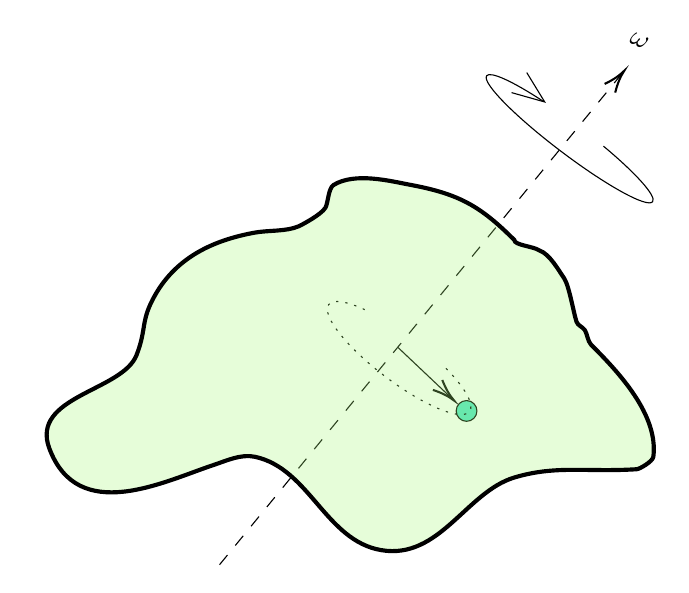
\begin{tikzpicture}[x=0.75pt,y=0.75pt,yscale=-1,xscale=1]
%uncomment if require: \path (0,300); %set diagram left start at 0, and has height of 300

%Straight Lines [id:da1466264621432246] 
\draw  [dash pattern={on 4.5pt off 4.5pt}]  (161,269.63) -- (354.73,33.18) ;
\draw [shift={(356,31.63)}, rotate = 129.33] [color={rgb, 255:red, 0; green, 0; blue, 0 }  ][line width=0.75]    (10.93,-3.29) .. controls (6.95,-1.4) and (3.31,-0.3) .. (0,0) .. controls (3.31,0.3) and (6.95,1.4) .. (10.93,3.29)   ;
%Shape: Arc [id:dp5966527947933914] 
\draw  [draw opacity=0] (345.95,67.97) .. controls (361.58,81) and (371.64,92.13) .. (369.66,94.74) .. controls (367.21,97.97) and (347.32,87) .. (325.24,70.25) .. controls (303.15,53.49) and (287.24,37.29) .. (289.69,34.06) .. controls (291.47,31.72) and (302.46,36.86) .. (316.8,46.28) -- (329.67,64.4) -- cycle ; \draw   (345.95,67.97) .. controls (361.58,81) and (371.64,92.13) .. (369.66,94.74) .. controls (367.21,97.97) and (347.32,87) .. (325.24,70.25) .. controls (303.15,53.49) and (287.24,37.29) .. (289.69,34.06) .. controls (291.47,31.72) and (302.46,36.86) .. (316.8,46.28) ;  
\draw   (309,32.52) -- (317.66,46.69) -- (301.68,42.18) ;
%Straight Lines [id:da4118334667699356] 
\draw    (247,165) -- (272.55,189.18) ;
\draw [shift={(274,190.55)}, rotate = 223.42] [color={rgb, 255:red, 0; green, 0; blue, 0 }  ][line width=0.75]    (10.93,-3.29) .. controls (6.95,-1.4) and (3.31,-0.3) .. (0,0) .. controls (3.31,0.3) and (6.95,1.4) .. (10.93,3.29)   ;
%Shape: Circle [id:dp5534282668246396] 
\draw  [fill={rgb, 255:red, 80; green, 227; blue, 194 }  ,fill opacity=1 ] (275,195.55) .. controls (275,192.79) and (277.24,190.55) .. (280,190.55) .. controls (282.76,190.55) and (285,192.79) .. (285,195.55) .. controls (285,198.31) and (282.76,200.55) .. (280,200.55) .. controls (277.24,200.55) and (275,198.31) .. (275,195.55) -- cycle ;
%Shape: Arc [id:dp400640896970585] 
\draw  [draw opacity=0][dash pattern={on 0.84pt off 2.51pt}] (270.08,175) .. controls (279.21,184.33) and (283.96,192.49) .. (281.44,195.8) .. controls (277.72,200.7) and (259.52,193.15) .. (240.78,178.93) .. controls (222.04,164.72) and (209.86,149.22) .. (213.58,144.31) .. controls (215.66,141.57) and (222.27,142.72) .. (230.96,146.75) -- (247.51,170.06) -- cycle ; \draw  [dash pattern={on 0.84pt off 2.51pt}] (270.08,175) .. controls (279.21,184.33) and (283.96,192.49) .. (281.44,195.8) .. controls (277.72,200.7) and (259.52,193.15) .. (240.78,178.93) .. controls (222.04,164.72) and (209.86,149.22) .. (213.58,144.31) .. controls (215.66,141.57) and (222.27,142.72) .. (230.96,146.75) ;  
%Shape: Boxed Bezier Curve [id:dp9065187303448061] 
\draw [fill={rgb, 255:red, 167; green, 247; blue, 120 }  ,fill opacity=0.28 ][line width=1.5]    (303,113.17) .. controls (286.54,96.7) and (276.25,90.99) .. (253,86.63) .. controls (243.19,84.79) and (226.35,80.42) .. (216,86.63) .. controls (213.32,88.24) and (213.34,95.4) .. (212,97.63) .. controls (209.91,101.11) and (200.15,106.14) .. (199,106.63) .. controls (193.13,109.15) and (184.49,108.45) .. (178,109.63) .. controls (158.17,113.24) and (140.45,121.35) .. (130,139.63) .. controls (122.75,152.32) and (126.06,155.61) .. (121,168.63) .. controls (114.22,186.06) and (69.55,188.44) .. (79,213.63) .. controls (92.8,250.44) and (133.8,229.7) .. (158,221.63) .. controls (164.45,219.48) and (171.35,216.21) .. (178,217.63) .. controls (204.4,223.29) and (212.04,258.14) .. (239,262.63) .. controls (266.99,267.3) and (279.92,234.56) .. (303,227.63) .. controls (323.23,221.56) and (337.72,225.15) .. (362,223.63) .. controls (363.34,223.55) and (369.72,219.9) .. (370,217.63) .. controls (372.54,197.3) and (353.17,176.81) .. (340,163.63) .. controls (338.35,161.98) and (338.13,158.33) .. (337,156.63) .. controls (335.95,155.06) and (333.6,154.42) .. (333,152.63) .. controls (331.57,148.33) and (329.39,135.09) .. (327,131.63) .. controls (324.44,127.93) and (320.04,119.85) .. (315,118.17) .. controls (312,116.17) and (303,115.73) .. (303,113.17) -- cycle ;

% Text Node
\draw (359.85,11.16) node [anchor=north west][inner sep=0.75pt]  [rotate=-24.91]  {$\omega $};


\end{tikzpicture}

    \caption{A rigid body rotating about an axis}
\end{figure}
\noindent
Consider a rigid body made of tiny masses $dm$. Consider one such mass sitauted as a distance $s$ from the fixed axis of rotation. It goes around a circle with speed $v = \omega s$. The angular momentum can be calculated as:
$$\mathbf{L} = \int (\veb{r}\times \veb{v})dm = \int (\veb{r}\times (\veb{\omega}\times \veb{r}))dm = \int (\veb{r}\cdot \veb{r})\veb{\omega} -  \cancelto{0}{(\veb{r}\cdot \veb{\omega})}\veb{r}dm =\veb{\omega} \underbrace{\int s^2 dm}_{\text{I}} $$
The integral is called the moment of inertia. In a more general case, where there is no fixed axis of rotation, we write: 
\begin{align*}
    \mathbf{L} &= \int (\veb{r}\times \veb{v})dm \\
    &= \int (\veb{r}\times (\veb{\omega}\times \veb{r}))dm \\
    &= \int (\veb{r}\cdot \veb{r})\veb{\omega} -  {(\veb{r}\cdot \veb{\omega})}\veb{r}dm
\end{align*}
We now write it in index notation, noting that $\omega^i = \tensor*{\delta}{^i^j}\omega_j$:
\begin{align*}
    L^i &= \int (\veb{r}\cdot \veb{r})\tensor*{\delta}{^i^j}\omega_j - x^i(x^j\omega_j)dm\\
    &= \omega_j \brac{\int (\veb{r}\cdot \veb{r})\tensor*{\delta}{^i^j} - x^ix^j\ dm} 
\end{align*}
The integral in the bracket is defined to be the inertia tensor:
$$I^{ij} = \int (\veb{r}\cdot \veb{r})\tensor*{\delta}{^i^j} - x^ix^j \ dm$$
Note that $i$ and $j$ goes from $1$ to $3$ and thus it has $9$ components but since the expression is symmetric, we only have $6$ independent components. This states that the angular momentum and the angular velocity are not necessarily parallel in some coordinate system where $I$ have non-zero off-diagonal entries.\\[0.3cm]
\textbf{Electromagnetic Tensor:}\\[0.3cm]
The electromagnetic tensor is very useful in combining the electric field and magnetic field and finding their transformations. It is defined as:
$$F_{\mu\nu} = \partial_\mu A_\nu - \partial_\nu A_\mu$$
where $A_\mu$ is the 4-potential. The indices $\mu$ and $\nu$ can take values from $0$ to $3$. The tensor has $16$ components but only $6$ of them are independent. The tensor is antisymmetric, that is, $F_{\mu\nu} = -F_{\nu\mu}$ and thus the diagonal entries are zero. We will discuss this later but Maxwell's equations can be written in a very compact form using the components of the electromagnetic tensor.\\[0.3cm]
\textbf{Electric-Susceptibility Tensor:}\\[0.3cm]
We had studied about polarisation in dielectrics in our classical electrodynamics course where we had often taken (for simplicity):
$$\veb{P} = \epsilon_0\chi\veb{E}$$
Here we had taken the electric field to be parallel to the polarisation vector but in general, these are related by the susceptibility tensor as:
$$P^i = \epsilon_0\chi^{ij}E^{j}$$
\subsection{Tensor Transformations}
As previously seen for vector transformation, the transformation of a tensor from one system to another is very similar. For simplicity, we show for a second rank tensor:
$$\tensor{T }{^{\prime ij}} = \pdv{x^{\prime i}}{x^k} \pdv{x^{\prime j}}{x^n} \tensor{T}{^{kn}}$$
This is simple: in the left everything is prime and contravariant, so in the right the numerator must have primes and the denominator must have unprimed indices and contraction should be done so as to match the contra and co indices on both sides in the final expansion. Well, this transformation law is such a nice thing that many people say that: 
$$\boxed{\mathrm{Tensors\ are \ defined\ in\ the\ way\ they\ transform}}$$
\subsection{Matrices vs. Tensor? same same but different....}
Not all matrices are second-rank tensors \emoji{expressionless}. Yes, the components of a second-rank tensor can be arranged in a matrix form but there are many matrices which do not transform according to the above equation. Take for example the following matrix, which we assume as a tensor:
$$[T^{lm}] \equiv \begin{pmatrix}
    (x^2)^2 & x^1x^2\\
    x^1x^2 & (x^2)^2
\end{pmatrix}$$
Note that the 2 outside the bracket is the power and inside the bracket is the index of the component. Then after rotation, we have the following relation:
\begin{align*}
    x'^1 &= x^1\cos\theta + x^2\sin\theta \\
    x'^2 &= -x^1\sin\theta + x^2\cos\theta
\end{align*}
Let us find $T^{'11}$ which according to the transformation rule, should be:
\begin{align*}
    T^{'11} &= \pdv{x'^1}{x^k} \pdv{x'^1}{x^n} T^{kn} \\
    &=\pdv{x'^1}{x^1} \pdv{x'^1}{x^1} T^{11} + \pdv{x'^1}{x^1} \pdv{x'^1}{x^2} T^{12}+\pdv{x'^1}{x^2} \pdv{x'^1}{x^1} T^{21} +\pdv{x'^1}{x^2} \pdv{x'^1}{x^2}T^{22}\\
    &= \cos\theta\cos\theta T^{11} + \cos\theta \sin\theta T^{12} + \sin\theta\cos\theta T^{21} + \sin\theta\sin\theta T^{22} \\
    &= \cos^2\theta (x^2)^2 + 2\sin\theta\cos\theta (x^1)(x^2) + \sin^2\theta (x^2)^2\\
    &=(x^2\cos\theta + x^1\sin\theta)^2
\end{align*}
Well note that if $T$ was indeed a tensor, then $T^{'11}$ should be equal to $(x'^2)^2$ but it is not. Thus, $T$ is not a tensor and our assumption was wrong.  \textbf{Thus all matrices are not tensors!}
\section{Metric Tensor: how yo mama's fatness is quantified!}
Let us consider the spherical polar coordinates $(r,\theta,\phi)$. Note that the coordinate displacement $d\phi$ does not have the dimension of length. So, while considering the displacement vector, we write $d\veb{r} \sim r\sin\theta d\phi \hat{\veb{\phi}}$. Thus, in general, for any displacement we write it in terms of the ``metric tensor'' $g^{ij}$ as:
$$ds^2 = g_{ij}x^ix^j$$
In rectangular coordinates, we have $g_{ij} = \delta_{ij}$, that is, the metric tensor is just the identity matrix. In cylindrical coordinates where $dx^1 = d\rho, dx^2 = d\phi, dx^3 = z$, we have:
$$g_{ij}= \begin{pmatrix}
    1 & 0 & 0\\
    0 & \rho^2 & 0\\
    0 & 0 & 1
\end{pmatrix}$$
Thus, the displacement is written as
$$ds^2 = g_{ij}dx^i dx^j = d\rho^2 + \rho^2 d\phi^2 + dz^2$$
In spherical polar coordinates, we have:
$$g_{ij} = \begin{pmatrix}
    1 & 0 & 0\\
    0 & r^2 & 0\\
    0 & 0 & r^2\sin^2\theta
\end{pmatrix}$$
Thus, the displacement is written as:
$$ds^2 = d\theta^2 + r^2 d\phi^2 + r^2\sin^2\theta d\phi^2$$
If all of $g_{ij}$ are non-negative we call that geometry ``Riemannian'' and if some of them are negative, it is termed ``pseudo-Riemannian''.\\[0.3cm]
\textbf{Now, how the hell do we calculate the components of the metric tensor?}\\[0.3cm]
Well we have previously seen how we could obtain the basis vectors using the partial derivatives of the coordinates. So, suppose we have to find the metric tensor for spherical polar coordinate system. For that, let us first write the position vector:
$$\veb{r} = x \veb{e}_x+y \veb{e}_y+z \veb{e}_z = r \sin\theta \cos\phi \ \veb{e}_x + r \sin\theta \sin\phi \ \veb{e}_y + r \cos\theta \ \veb{e}_z$$
From this we obtain:
\begin{align*}
    \veb{e}_r &= \pdv{\veb{r}}{r} =  \sin\theta \cos\phi \ \veb{e}_x + \sin\theta \sin\phi \ \veb{e}_y + \cos\theta \ \veb{e}_z\\
    \veb{e}_\theta &= \pdv{\veb{r}}{\theta} = r \cos\theta \cos\phi \ \veb{e}_x + r \cos\theta \sin\phi \ \veb{e}_y - r \sin\theta \ \veb{e}_z\\
    \veb{e}_\phi &= \pdv{\veb{r}}{\phi} = -r \sin\theta \sin\phi \ \veb{e}_x + r \sin\theta \cos\phi \ \veb{e}_y
\end{align*}
Now, we had defined the metric tensor components to be the scalar product of the basis vectors. Also note that since the basis vectors are orthogonal, there will be no cross terms, so the tensor is diagonal. Using this we have:
\begin{align*}
    g_{rr} &= \veb{e}_r\cdot \veb{e}_r = \sin^2\theta \cos^2\phi + \sin^2\theta \sin^2\phi + \cos^2\theta = 1\\
    g_{\theta\theta} &= \veb{e}_\theta\cdot \veb{e}_\theta = r^2 \cos^2\theta \cos^2\phi + r^2 \cos^2\theta \sin^2\phi + r^2 \sin^2\theta = r^2\\
    g_{\phi\phi} &= \veb{e}_\phi\cdot \veb{e}_\phi = r^2 \sin^2\theta \sin^2\phi + r^2 \sin^2\theta \cos^2\phi = r^2 \sin^2\theta
\end{align*}
This is exactly what we had written before. Thus using this procedure, we can easily find the components of the metric tensor and then just chill! 
\subsection{Metric in relativity:}
We now consider the case of Minkowski space, where the coordinate displacements between two events are described by four component vector (\textbf{4 vector}):
$$dx^\mu = (dt, dx,dy,dz)\equiv (dt, d\veb{r})$$
The spacetime interval can be written in terms of the metric tensor $g_{\mu\nu}$ as:
$$ds^2 = dt^2-dx^2-dy^2-dz^2= g_{\mu\nu} dx^\mu dx^\nu$$
Thus in this case the metric tensor is:
$$g_{\mu\nu} = \begin{pmatrix}
    1 & 0 & 0 & 0\\
     1 & -1 & 0 & 0\\
      1 & 0 & -1 & 0\\
       1 & 0 & 0 & -1\\
\end{pmatrix}$$
Note the convention. Other conventions include the obnoxious $(+,-,-,-)$ or the $(+,+,+,+)$ with an imaginary time. The overall thing is, spatial and temporal part should have some difference.\\[0.3cm] We also define the ``proper time'' as $d\tau = \frac{ds}{c}$. Since we take $c=1$, then both are equivalent but let's take $c$ to be $c$ for once. Then,
$$c^2 d\tau^2 = c^2dt^2-dx^2-dy^2-dz^2 = c^2dt^2\brac{1 - \frac{dx^2+dy^2+dz^2}{c^2dt^2}} = c^2dt^2\brac{1-\frac{v^2}{c^2}}$$
From this we have
$$\boxed{\dv{\tau}{t} = \sqrt{1- \frac{v^2}{c^2}}:=\gamma}$$


\section{Tensor Derivatives: levelling up the rizz!}
Till now, we had just seen the transformation of tensors and tensor densities. However, an important aspect of any calculation is the ability to take derivatives \footnote{A person's intellectual prowess can be judged their ability to take derivatives \emoji{smiling-face-with-sunglasses}}. Derivatives occur everywhere in calculations and we need a way to tackle them. So let's start\dots

\subsection{Velocity}
Well velocity is a vector (we had been reminded many a times) and it should then transform as a vector. Now, 
we know the transformation:
$$dx'^i = \pdv{x'^i}{x^l}x^l$$
To find velocity components, we have to differentiate with respect to time $t$. 
\begin{align*}
    \dv{x'^i}{t} &= \dv{t}\brac{\pdv{x'^i}{x^l}x^l}\\
    &=\pdv{x'^i}{x^l}\dv{x^l}{t} + x^l \dv{t}\brac{\pdv{x'^i}{x^l}}\\
    &=\pdv{x'^i}{x^l}\dv{x^l}{t} + x^l \pdv{x'^i}{x^k}{x^l}\dv{x^k}{t}
\end{align*}
Now we define $v^k = \dv{x^k}{t}$. Then the above expression would give:
\begin{align*}
    v'^i = \pdv{x'^i}{x^l}v^l +  \pdv{x'^i}{x^k}{x^l}x^l v^k
\end{align*}
The first term gives the proper thing for velocity to be a vector, like the correct transformation. The second term is the BAD term \emoji{face-with-steam-from-nose}. Let's see some examples of this term in some transformation:\\[0.3cm]
\textbf{Rotation:}
\begin{align*}
    x' &= x\cos\theta+y\sin\theta\\
    y'&=-x\sin\theta + y\cos\theta
\end{align*}
So we have: 
\begin{align*}
    \pdv{x'}{x} = \cos\theta \quad  \pdv{x'}{y} = \sin\theta \quad  \pdv{y'}{x} = -\sin\theta \quad
    \pdv{y'}{y} = \cos\theta
\end{align*}
Note that the first derivatives do not depend on the coordinate anymore. For a fixed $\theta$, the first derivatives are constants. 
And if we consider the transformation of the velocity components, then the second term will vanish, since these contain double derivatives. Thus, the BAD term vanishes and we happily see that velocity is a vector under rotation. In Galilean transformation ($x'=x-vt, y'=y, z'=z, t'=t$) too, the second term vanish. Even in Lorentz transformation ($t' = \gamma \brac{t-vx}, x=\gamma(x-vt), y'=y, z'=z$) the bad term vanishes. So in basic transformations, velocity is indeed a vector. Let us now see how derivative of a tensor component transforms. So we have,
\begin{align*}
    (\partial_\lambda T^\alpha)' = \partial_{\lambda'}\mathcolor{red}{T'^\lambda}&= \mathcolor{blue}{\frac{\partial}{\partial x'^\lambda}}\brac{\mathcolor{red}{\pdv{x'\lambda}{x^\sigma}T^\sigma}} \quad \ \ (\text{contravariant transformation of tensor})\\
    &= \mathcolor{blue}{\pdv{x^\rho}{x'^\lambda}\frac{\partial}{\partial x^\rho}}\brac{{\pdv{x'^\lambda}{x^\sigma}T^\sigma}}\quad \ \ (\text{covariant transformation of derivative})\\
    &= \pdv{x^\rho}{x'^\lambda}\pdv{x'^\alpha}{x^\sigma}\partial_\rho T^\sigma + \pdv{x^\rho}{x'^\lambda}\pdv{x'^\alpha}{x^\rho}{x^\sigma}T^\sigma \quad \ \ (\text{chain rule})
\end{align*}
Again, the first term is the usual thing but the BAD term appears again! Notice how always the bad term contains a double derivative. Now we know that double derivatives have something to do with curvatures. Let us clarify a bit more.\\[0.3cm]
Imagine the position vector $\veb{r}(t)$ on a flat space. Then the tangent vector to a point having position $\veb{r}(t)$, say $\veb{v}$, will lie entirely on the same space, right? But now, imagine the space being curved. Now if we draw the tangent, it will inevitable leave the space. Imagine the people living on the surface of a sphere. The velocity vector for a moving body in the space will be tangent to the sphere and points off of it. So, for the inhabitants, the velocity vector doesn't exist since it is not contained entirely on the space (Is this the same case with \textit{God}? Hmm, something to think about \emoji{thinking}). What they can do it, just take some small patch of the sphere (which is flat) where the tangent touches the surface and around it, locally, they can define the velocity vector. So, in general the velocity is not a tensor in curved space, where the second derivative is non-zero. 

% \begin{figure}[H]
%     \centering 
%     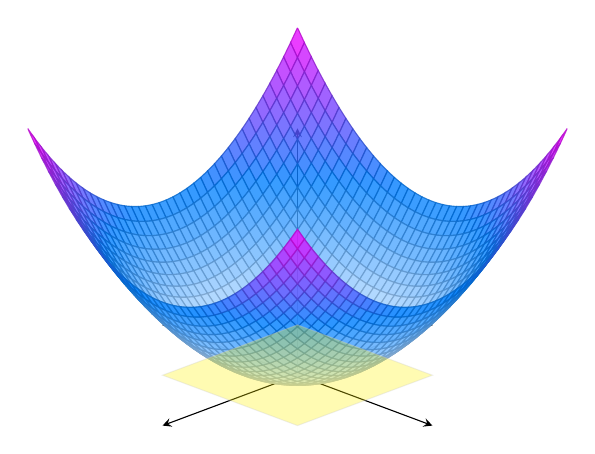
\begin{tikzpicture}
  \begin{axis}[
      view={135}{30},
      colormap/cool,
      axis lines=center,
      xlabel={}, ylabel={}, zlabel={},
      domain=-2:2,
      y domain=-2:2,
      samples=40,
      samples y=40,xtick=\empty,
ytick=\empty,
ztick=\empty
    ]

    % Paraboloid surface z = x^2 + y^2
    \addplot3[
      surf,
      opacity=0.8
    ]
    {x^2 + y^2};

    % Tangent plane at origin z = 0
    \addplot3 [
      surf,
      domain=-1:1,
      y domain=-1:1,
      samples=2,
      samples y=2,
      fill=yellow,
      opacity=0.3
    ]
    {0};

  
   

  \end{axis}
\end{tikzpicture}
%     \caption{Notice how all the tangents at the lowest point of the paraboloid $(x=0,y=0)$ is constrained to be in the yellow coloured plane. Now only some area around $x=0,y=0$ can be made to look locally like the yellow plane and hence the definition of velocity will be valid only locally, within that patch.   }
% \end{figure}
\subsection{Affine Connection}
Suppose in a locally inertial frame, for an object we have zero acceleration, that is:
$$\dv[2]{X^\alpha}{\uptau} = 0$$
Suppose the coordinates $X^\alpha \equiv X^\alpha(x^\mu)$ where $x^\mu$ are coordinates of a ground-based inertial reference frame relative to which the object accelerates. Then using chain rule, we have from the previous relation:
$$\frac{d}{d\uptau}\brac{\pdv{X^\alpha}{x^\mu}\dv{x^\mu}{\uptau}} = 0$$

Using product rule and chain rule again, we have:
$$\pdv{X^\alpha}{x^\mu}\dv[2]{x^\mu}{\uptau} +\pdv{X^\alpha}{x^\mu}{x^\rho} \dv{x^\rho}{\uptau} \dv{x^\mu}{\uptau}=0$$
Now we do one nice thing: multiply the above with $\pdv{x^\lambda}{X^\alpha}$:
$$\pdv{x^\lambda}{X^\alpha}\brac{\pdv{X^\alpha}{x^\mu}\dv[2]{x^\mu}{\uptau}} +\pdv{x^\lambda}{X^\alpha}\brac{\pdv{X^\alpha}{x^\mu}{x^\rho} \dv{x^\rho}{\uptau} \dv{x^\mu}{\uptau}}=0$$
Doing this, a nice thing occurs but for that we have to note that $\pdv{x^\lambda}{X^\alpha}\pdv{X^\alpha}{X^\mu} = \tensor{\delta}{^\lambda _\mu}$. Then from the first term, we get the kronecker delta and the expression reduces to:
$$\dv[2]{x^\lambda}{\uptau} +\mathcolor{blue}{\pdv{x^\lambda}{X^\alpha}\pdv{X^\alpha}{x^\mu}{x^\rho}} \dv{x^\rho}{\uptau} \dv{x^\mu}{\uptau}=0 \quad \implies \quad \dv[2]{x^\lambda}{\uptau} +\mathcolor{blue}{\tensor{\Gamma}{^\lambda _\mu _\rho}} \dv{x^\rho}{\uptau} \dv{x^\mu}{\uptau}=0$$
Here we have identified the scary blue term with a symbol with three indices, one upper and two lower (since in the blue term, there is one upper and two lower indices). This thing, we call the \textbf{affine connection}. 
Note that since derivatives commute\footnote{If a space has something called a `torsion', then the derivatives no longer commute and the following property does not hold true} generally, we have the lower indices of the affine connection to be symmetric, that is,
$$\tensor{\Gamma}{^\alpha _\mu _\nu} =\tensor{\Gamma}{^\alpha _\nu _\mu}$$
\subsubsection{Definition in terms of basis vectors}
We can define the affine connection using basis vectors also. Consider the derivative of the basis vector $\veb{e}_i$ with respect to some coordinates. This derivate is another vector which when expanded in terms of the basis, the coefficients are nothing but the affine connection. 
$$\pdv{\veb{e}_i}{x^j} = \tensor{\Gamma}{^k _{ij}}\veb{e}_k$$

\subsubsection{Transformation of Affine Connection}
Note that the affine connection contains both coordinates $X^\alpha$ and $x\mu$. Suppose we want to transform from $x$ to $x'$ coordinate system, then only the $x$ things will be changed, not the $X$ things. Leave the $X$ alone because the transformation being studied is specifically about how the connection coefficients behave when you change coordinate systems on the ground. So we have:
\begin{align*}
    \tensor{(\Gamma')}{^\lambda _\mu _\nu} &= \mathcolor{blue}{\pdv{x'^\lambda}{X^\alpha}}\pdv{X^\alpha}{x'^\mu}{x'^\nu}\\
    &= \mathcolor{blue}{\pdv{x'^\lambda}{x^\rho}\pdv{x^\rho}{X^\alpha}}\pdv{X^\alpha}{x'^\mu}{x'^\nu} \quad \text{(using chain rule )}\\
    &=\brac{\pdv{x'^\lambda}{x^\rho}\pdv{x^\rho}{X^\alpha}} \pdv{x'^\mu}\brac{\mathcolor{OliveGreen}{\pdv{X^\alpha}{x^\sigma}}\mathcolor{red}{ \pdv{x^\sigma}{x'^\nu}}} \quad \text{(using chain rule again )}\\
    &=\brac{\pdv{x'^\lambda}{x^\rho}\pdv{x^\rho}{X^\alpha}}\brac{ { \mathcolor{red}{\pdv{x^\sigma}{x'^\nu}}\pdv{x'^\mu}\brac{\mathcolor{OliveGreen}{\pdv{X^\alpha}{x^\sigma}}} + \mathcolor{OliveGreen}{\pdv{X^\alpha}{x^\sigma}}\pdv{\mathcolor{red}{x^\sigma}}{x'^\mu}{\mathcolor{red}{x'^\nu}}}}\quad \text{(using product rule )}\\
    &=\brac{\pdv{x'^\lambda}{x^\rho}\pdv{x^\rho}{X^\alpha}} \brac{\pdv{x^\sigma}{x'^\nu} \pdv{X^\alpha}{x^\kappa}{x^\sigma}\pdv{x^\kappa}{x'^\mu}+ \pdv{X^\alpha}{x^\sigma}\pdv{x^\sigma}{x'^\mu}{x'^\nu}}\quad \text{(using chain rule )}
\end{align*}
Well well, I know this was a shitty calculation but hey, sometimes shit is what relieves us! We now focus on the two terms separately in the above expression. 
\begin{itemize}
    \item \textbf{The First Term:} $\brac{\pdv{x'^\lambda}{x^\rho}\pdv{x^\rho}{X^\alpha}}\pdv{x^\sigma}{x'^\nu} \pdv{X^\alpha}{x^\kappa}{x^\sigma}\pdv{x^\kappa}{x'^\mu}$\\[0.3cm]
This can be rearranged a bit and can be written as 
$$   \brac{\pdv{x'^\lambda}{x^\rho}\pdv{x^\sigma}{x'^\nu} \pdv{x^\kappa}{x'^\mu}}   \brac{\pdv{x^\rho}{X^\alpha}\pdv{X^\alpha}{x^\kappa}{x^\sigma}} \equiv \brac{\pdv{x'^\lambda}{x^\rho}\pdv{x^\sigma}{x'^\nu} \pdv{x^\kappa}{x'^\mu}}  \tensor{\Gamma}{^\rho _\kappa _\sigma}$$
\item \textbf{The Second Term:} $\brac{\pdv{x'^\lambda}{x^\rho}\mathcolor{blue}{\pdv{x^\rho}{X^\alpha}}}\mathcolor{blue}{\pdv{X^\alpha}{x^\sigma}}\pdv{x^\sigma}{x'^\mu}{x'^\nu}$
The blue terms together gives $\tensor{\delta}{^\rho _\sigma}$ which reduces the expression to:
$$\pdv{x'^\lambda}{x^\rho}\pdv{x^\rho}{x'^\mu}{x'^\nu}$$
\end{itemize}
Thus, finally we obtain the expression for the transformation of the affine connection:
$$\boxed{ \tensor{(\Gamma')}{^\lambda _\mu _\nu} = \brac{\pdv{x'^\lambda}{x^\rho}\pdv{x^\sigma}{x'^\nu} \pdv{x^\kappa}{x'^\mu}}  \tensor{\Gamma}{^\rho _\kappa _\sigma} +\pdv{x'^\lambda}{x^\rho}\pdv{x^\rho}{x'^\mu}{x'^\nu} }$$
Note that the first term is the usual transformation rule for the affine connection but again the second BAD term emerges which, if non-zero, will lead to the affine connection not being a tensor.\\[0.3cm]
Now note that the BAD term contains the second derivative of the old coordinates with respect to the old coordinates, but generally we have the other way. So it would be a bit nice if we could change it. For that, note the identity and differentiate with respect to $x'^\mu$:
\begin{align*}
   &\pdv{x'^\lambda}{x^\rho}\pdv{x^\rho}{x'^\nu}=\tensor{\delta}{^\lambda_\nu}\\
\implies & \pdv{x'^\mu}\brac{\pdv{x'^\lambda}{x^\rho}\pdv{x^\rho}{x'^\nu}}=0\\
\implies & \brac{\pdv{x'^\lambda}{x^\rho}} \brac{\pdv{x^\rho}{x'^\nu}{x'^\mu} }+ \brac{\pdv{x^\rho}{x'^\nu}}\brac{\pdv{x'^\lambda}{x^\rho}{x'^\mu}}=0\\
\implies & \brac{\pdv{x'^\lambda}{x^\rho}} \brac{\pdv{x^\rho}{x'^\nu}{x'^\mu} } + \brac{\pdv{x^\rho}{x'^\nu}}\brac{\pdv{x'^\lambda}{x^\rho}{x^\sigma}\pdv{x^\sigma}{x'^\mu}}=0
\end{align*}
The first term in the above is exactly the BAD term in the affine connection transformation and thus we replace this. Then we have: 
$$\boxed{ \tensor{(\Gamma')}{^\lambda _\mu _\nu} = \brac{\pdv{x'^\lambda}{x^\rho}\pdv{x^\sigma}{x'^\nu} \pdv{x^\kappa}{x'^\mu}}  \tensor{\Gamma}{^\rho _\kappa _\sigma} - \brac{\pdv{x^\rho}{x'^\nu}}\brac{\pdv{x'^\lambda}{x^\rho}{x^\sigma}\pdv{x^\sigma}{x'^\mu}} }$$
\subsection{Covariant Derivatives}
In every transformation seen so far, we had got a BAD term (containing a second derivative) which spoils the transformation. So wouldn't it be nice if we just redefine the definition of a derivative so that this BAD term gets cancelled from the definition only? This brings us to \textit{covariant derivative} 
\\[0.3cm]
\textbf{A Notational Nightmare:}\\[0.3cm]
The symbol of covariant derivative is very confusing. Different people use different notation for it. Some use $D$ for it, some use $\nabla$ while some use $;$. We will use $;$ for it, I guess but we may sometimes shift to $D$ notation if ambiguity arises...\\[0.3cm]
The covariant derivative of a vector component with respect to a scalar is defined as:
$$\frac{DA^\lambda}{D\uptau} := \frac{dA^\lambda}{d\uptau}+ \tensor{\Gamma}{^\lambda _\mu _\nu}\dv{x^\mu}{\uptau}A^\nu$$
Here we used the $D$ notation since the $;$ notation is mostly used when we differentiate with respect to some coordinate. The covariant derivative of a vector component with respect to a coordinate is then\footnote{$\tensor{A}{^\nu _, _\mu}$ means the normal derivative, that is, $\partial_\mu A^\nu$}: 
$$\tensor{A}{^\lambda _; _\mu} :=  \tensor{A}{^\lambda _, _\mu} +\tensor{\Gamma}{^\lambda _\mu _\nu}A^\nu$$
The covariant derivative of a covariant component is similarly defined:
$$\tensor{A}{_\lambda _; _\mu} :=  \tensor{A}{_\lambda _, _\mu} +\tensor{\Gamma}{^\alpha _\lambda _\nu}A_\alpha$$
\subsubsection{Transformation of Covariant Derivative}
In the primed frame, we have: 
\begin{align*}
\tensor{{A'}}{^\lambda _{;\uptau}} &= \tensor{{A'}}{^\lambda _{,\uptau}} + \tensor{{\Gamma'}}{^\lambda _{\mu \nu}} \dv{x'^\mu}{\uptau} \tensor{{A'}}{^\nu} \\
&= \left( \pdv{x'^\lambda}{x^l} \dv{A^l}{\uptau} 
+ A^l \pdv{x'^\lambda}{x^k}{x^l} \dv{x^k}{\uptau} \right) \\
&\quad + \Bigg[ 
\brac{\pdv{x'^\lambda}{x^\rho}\pdv{{x^\sigma}}{{x'^\nu}} \pdv{{x^\kappa}}{{x'^\mu}}}  \tensor{\Gamma}{^\rho _\kappa _\sigma} - \brac{\pdv{{x^\rho}}{{x'^\nu}}}\brac{\pdv{x'^\lambda}{x^\rho}{x^\sigma}\pdv{{x^\sigma}}{{x'^\mu}}}  \Bigg]
 \\
&\qquad \times \left( 
\pdv{x'^\mu}{x^\omega} \dv{x^\omega}{\uptau} 
+ x^\omega \pdv[2]{x'^\mu}{x^\omega}{x^\beta} \dv{x^\beta}{\uptau} 
\right)
\pdv{{x'^\nu}}{{x^\theta}} A^\theta
\end{align*}
Let's see this term by term. 
\begin{itemize}
    \item \textbf{The First Term:} Transformation of normal derivative 
    $$ \boxed{\pdv{x'^\lambda}{x^l} \dv{A^l}{\uptau} }
+ \mathcolor{OliveGreen}{A^l \pdv{x'^\lambda}{x^q}{x^l} \dv{x^q}{\uptau}}$$
This is fine for now. Let's leave it here!
    \item \textbf{The Second Term:} Multiplication of three individual terms
    Well, this is the monster \emoji{alien-monster} actually. When expanded, it will have four terms. Let us write them one by one: 
    \begin{enumerate}
        \item After reducing the Kronecker delta, the final expression becomes: \begin{align*} 
            \pdv{x'^\lambda}{x^\rho}\pdv{{x^\sigma}}{\mathcolor{blue}{x'^\nu}} \pdv{{x^\kappa}}{\mathcolor{purple}{x'^\mu}}\pdv{\mathcolor{blue}{x'^\nu}}{x^\theta}\pdv{\mathcolor{purple}{x'^\mu}}{x^\omega}\dv{x^\omega}{\uptau}\tensor{\Gamma}{^\rho _\kappa _\sigma}A^\theta =\boxed{\pdv{x'^\lambda}{x^\rho}\dv{x^\kappa}{\uptau}\tensor{\Gamma}{^\rho _\kappa _\sigma}A^\sigma}
        \end{align*}
        \item After reducing the Kronecker delta, we have:
        \begin{align*}
            - {\pdv{{x^\rho}}{\mathcolor{blue}{x'^\nu}}}{\pdv{x'^\lambda}{x^\rho}{x^\sigma}\pdv{{x^\sigma}}{{\mathcolor{red}{{x'^\mu}}}}}\pdv{\mathcolor{blue}{x'^\nu}}{x^\theta}\pdv{\mathcolor{red}{x'^\mu}}{x^\omega}\dv{x^\omega}{\uptau}A^\theta = -\mathcolor{OliveGreen}{\pdv{x'^\lambda}{x^\rho}{x^\sigma} \dv{x^\sigma}{\uptau}A^\rho}
        \end{align*}
        Note this final term and the \textbf{first term}, both of these differ only by the fact that $q\rightarrow \sigma$ and $l \rightarrow \rho$ but since these are dummy indices, we can just rename them and these terms are actually equal but we have a minus sign in this term, so this cancels with the first term. 
        \item After reducing the Kronecker delta, we have:
        \begin{align*}
            \pdv{x'^\lambda}{x^\rho} \pdv{x^\kappa}{x'^\mu} \pdv{x'^\sigma}{\mathcolor{purple}{x'^\nu}} \pdv{\mathcolor{purple}{x'^\nu}}{x^\theta} \pdv{x'^\mu}{x^\omega}{x^\beta} \dv{x^\beta}{\uptau} x^\omega \tensor{\Gamma}{^\rho_\kappa _\sigma} A^\theta = \pdv{x'^\lambda}{x^\rho} \pdv{x^\kappa}{x'^\mu} \pdv{x'^\mu}{x^\omega}{x^\beta} \dv{x^\beta}{\uptau} x^\omega \tensor{\Gamma}{^\rho_\kappa _\sigma} A^\sigma
        \end{align*}
        \item Same, after reducing the Kronecker delta, we have: \begin{align*}
           - \pdv{x^\sigma}{x'^\mu} \pdv{x^\rho}{\mathcolor{cyan}{x'^\nu}} \pdv{\mathcolor{cyan}{x'^\nu}}{x^\theta} \pdv{x'^\lambda}{x^\rho}{x^\sigma}\pdv{x'^\mu}{x^\omega}{x^\beta} \dv{x^\beta}{\uptau} x^\omega  A^\theta = -\pdv{x^\sigma}{x'^\mu}  \pdv{x'^\lambda}{x^\rho}{x^\sigma}\pdv{x'^\mu}{x^\omega}{x^\beta} \dv{x^\beta}{\uptau} x^\omega  A^\rho
        \end{align*}
    \end{enumerate}
\end{itemize}
Okay, so the green terms cancel and note the boxed terms, these are actually the terms which should have been in the transformation equation of covariant derivative, if it were a tensor. So, let us now focus on the remaining terms, that is, the last two terms. Note the third term:
\begin{align*}
    \pdv{x'^\lambda}{x^\rho} \pdv{x^\kappa}{x'^\mu} \pdv{x'^\mu}{x^\omega}{x^\beta} \dv{x^\beta}{\uptau} x^\omega \brac{\tensor{\Gamma}{^\rho_\kappa _\sigma}} A^\sigma &= \pdv{x'^\lambda}{\mathcolor{cyan}{x^\rho}} \pdv{x^\kappa}{x'^\mu} \pdv{x'^\mu}{x^\omega}{x^\beta} \dv{x^\beta}{\uptau} \brac{\pdv{\mathcolor{cyan}{x^\rho}}{x'^\gamma}\pdv{x'^\gamma}{x^\kappa}{x^\sigma}}x^\omega A^\sigma \\
    &= \pdv{x^\kappa}{x'^\mu} \pdv{x'^\mu}{x^\omega}{x^\beta} \dv{x^\beta}{\uptau} \pdv{x'^\lambda}{x^\kappa}{x^\sigma}x^\omega A^\sigma
\end{align*}
We had just replaced the affine connection coefficient and reduced the kronecker delta. Then this turns into the fourth term ($\rho \rightarrow \sigma$ and $\sigma \rightarrow \kappa$) and hence these two terms cancel. Then we remain only with the boxed terms and hence the covariant derivative with respect to a scalar actually transforms as a vector. 
$$\tensor{{A'}}{^\lambda _{;\uptau}} = \pdv{x'^\lambda}{x^\rho} \dv{A^\rho}{\uptau} +\pdv{x'^\lambda}{x^\rho}\dv{x^\kappa}{\uptau}\tensor{\Gamma}{^\rho _\kappa _\sigma}A^\sigma =  \pdv{x'^\lambda}{x^\rho}\brac{\dv{A^\rho}{\uptau}+\dv{x^\kappa}{\uptau}\tensor{\Gamma}{^\rho _\kappa _\sigma}A^\sigma} = \pdv{x'^\lambda}{x^\rho} \dv{A^\rho}{\uptau}\tensor{A}{^\rho _; _\uptau}$$
We saw how \textit{easy} it was to show the transformation of covariant derivative. It's going to get easier as we progress. Now, similar to the above, we can show that the covariant derivative with respect to a coordinate is a second-rank tensor. 
$$\tensor{{A'}}{^\lambda _{;\mu}} =\pdv{x'^\lambda}{x^\rho} \pdv{x^\sigma}{x'^\mu}\tensor{A}{^\rho _; _\mu}$$
The covariant derivative of a general tensor is given by the following formula:
$$\tensor{A}{^{i_1\ldots i_r} _{j_1\ldots j_s;p}} = \tensor{A}{^{i_1\ldots i_r} _{j_1\ldots j_s,p}} + 
\sum\limits_{u=1}^r \tensor{\Gamma}{^{i_u} _{h_u p}}\tensor{A}{^{i_1\ldots i_{u-1}h_u i_{u+1}\ldots i_r} _{j_1\ldots j_s}} - \sum\limits_{u=1}^s \tensor{A}{^{i_1\ldots i_r} _{j_1 \ldots j_{u-1}h_u j_{u+1}\ldots j_s}}\tensor{\Gamma}{^{h_u} _{j_u p}}$$
Basically, the first term is the conventional derivative. For all the contravariant indices, we have $+$ sign while for covariant indices, we have $-$ sign. And in each sum, remove the $u^{\text{th}}$ index and replace it with an arbitrary variable in the tensor and then accordingly adjust the affine connection. Let us see some examples perhaps, using this formula:
\begin{align*}
    \tensor{T}{^\mu ^\nu _{;\beta}} &= \tensor{T}{^\mu ^\nu _{,\beta}} + \tensor{\Gamma}{^\mu _\kappa _\beta}\tensor{T}{^\kappa ^\nu} + \tensor{\Gamma}{^\nu _\kappa _\beta}\tensor{T}{^\mu ^\kappa}\\
\tensor{T}{^\mu ^\nu _{\sigma;\beta}} &= \tensor{T}{^\mu ^\nu _{\sigma,\beta}} + \tensor{\Gamma}{^\mu _\kappa _\beta}\tensor{T}{^\kappa ^\nu _\sigma} + \tensor{\Gamma}{^\nu _\kappa _\beta}\tensor{T}{^\mu ^\kappa _\sigma} - \tensor{\Gamma}{^\kappa _{\sigma \beta}}\tensor{A}{^{\mu \nu} _\kappa}
\end{align*}
\subsubsection{Covariant Derivatives using Basis Vectors}

\begin{theorem}[Product Rule]
    The covariant derivative satisfies a kind of product rule like: 
    \[
\tensor{(A^\nu B^\mu)}{_{;\alpha}} = \tensor{A}{^\nu} \tensor{B}{^\mu _{;\alpha}} + \tensor{B}{^\mu} \tensor{A}{^\nu _{;\alpha}}
\]

\end{theorem}
\textit{Proof.} We show it for a rank two contravariant tensor. We begin with the usual expansion of the covariant derivative:
\begin{align*}
    \tensor{(A^\nu B^\mu)}{_{;\alpha}} &=   \partial_\alpha(A^\nu B^\mu) + \tensor{\Gamma}{^\nu _{\kappa \alpha}}A^\kappa B^\mu +\tensor{\Gamma}{^\mu _{\kappa \alpha}}A^\nu B^\kappa  \\
    &= B^\mu \partial_\alpha A^\nu +  A^\nu \partial_\alpha B^\mu  + \tensor{\Gamma}{^\nu _{\kappa \alpha}}A^\kappa B^\mu +\tensor{\Gamma}{^\mu _{\kappa \alpha}}A^\nu B^\kappa\\
    &=B^\mu\brac{\partial_\alpha A^\nu  + \tensor{\Gamma}{^\nu _{\kappa \alpha}}A^\kappa} + A^\nu \brac{\partial_\alpha B^\mu +\tensor{\Gamma}{^\mu _{\kappa \alpha}} B^\kappa}\\
    &= \tensor{B}{^\mu} \tensor{A}{^\nu _{;\alpha}} + \tensor{A}{^\nu} \tensor{B}{^\mu _{;\alpha}}
\end{align*}
This can be generalised to higher rank tensor with mixed indices as well. 
% \begin{theorem}[Metric Compatibility]
%     The covariant derivative of the metric tensor is identically zero
%     $$g_{\mu\nu ; \alpha} = 0$$
% \end{theorem}
% \textit{Proof.} So from the above expression, we can write the covariant derivative of the metric tensor as: 
% $$g_{\mu\nu ; \alpha} = g_{\mu\nu , \alpha} - \tensor{\Gamma}{^\kappa _{\mu \alpha}} g_{\kappa \nu} - \tensor{\Gamma}{^\kappa  _\nu _\alpha} g_{\mu \kappa}$$ 
% Let us start with an arbitrary vector $v^\nu$. Then we have: 
% $$\tensor{v}{_\nu _{;\alpha}} = \tensor{{g_{\lambda \nu}v}}{^{\lambda} _{;\alpha}} = g_{\lambda \nu}( \tensor{v}{^{\lambda} _{;\alpha}}) +v^\lambda(\tensor{{g_{\lambda \nu}}}{ _{;\alpha}}) $$
% Now, consider the following where the unprimed indices denote Cartesian system and primed ones represent arbitrary system. Then we have the following valid in any coordinate system:
% $$v_{\alpha'} = g_{\alpha'\mu'}v^{\mu '}$$
% since it is a tensor equation. However, in Cartesian system, since metric tensor is identity, we have $V_\alpha = V^\alpha$. Also, the affine connection vanishes, hence the covariant and normal derivatives become same. So, using the above facts, in Cartesian coordinates, we have:
% \[
% \tensor{v}{^\alpha _{;\beta}} = \tensor{v}{^\alpha _{,\beta}} = \tensor{v}{_\alpha _{,\beta}} = \tensor{v}{_\alpha _{;\beta}} = \tensor{{g_{\alpha \mu}v^\mu}}{ _{;\beta}}
% \]

\subsection{Relating metric and affine connection}
% Let us write the transformation of the metric tensor. 
% $$g'_{\mu \nu} = \pdv{x^\rho}{x'^\mu}\pdv{x^\sigma}{x'^\nu}g_{\rho\sigma}$$
% And now comes the scary part, differentiate this expression with respect to some coordinate in the new frame:
% $$\pdv{x'^\kappa}\brac{\pdv{x^\rho}{x'^\mu}\pdv{x^\sigma}{x'^\nu}g_{\rho\sigma}} = \pdv{x^\rho}{x'^\mu}{x'^\kappa}\pdv{x^\sigma}{x'^\nu}g_{\rho\sigma}+\pdv{x^\rho}{x'^\mu}\pdv{x^\sigma}{x'^\nu}{x'^\kappa}g_{\rho\sigma}+\pdv{x^\rho}{x'^\mu}\pdv{x^\sigma}{x'^\nu}\partial_{\kappa'}g_{\rho\sigma}$$
% We write this in brief, as: 
% $$\partial_{\kappa '}g'_{\mu\nu} = ( \ \ldots\ )\partial_{\nu'}x^\sigma g_{\rho\sigma} +\partial_{\mu'}x^\rho( \ \ldots\ )g_{\rho\sigma} +\partial_{\nu'}x^\sigma\partial_{\mu'}x^\rho \partial_{\kappa '}g_{\rho\sigma}$$


% \noindent
% Now let us follow some steps blindly, which will lead to a result: 
% \begin{itemize}
%     \item We include two more expressions, pertaining to the permutations of these symbols. We then have three equations: 
% \begin{align*}
%     \partial_{\mu'}g'_{\kappa\nu} &= \partial_{\nu'}x^\sigma\frac{\partial^2 x^\rho}{\partial x'^{\kappa}\partial x'^{\mu}}g_{\rho\sigma} + \frac{\partial^2 x^\sigma}{\partial x'^{\nu}\partial x'^{\mu}}\partial_{\kappa'}x^\rho g_{\rho\sigma} + \partial_{\nu'}x^\sigma \partial_{\kappa'}x^\rho\partial_{\mu'}g_{\rho\sigma}\\
%      \partial_{\nu'}g'_{\kappa\mu} &= \partial_{\mu'}x^\sigma\frac{\partial^2 x^\rho}{\partial x'^{\kappa}\partial x'^{\nu}}g_{\rho\sigma} + \frac{\partial^2 x^\sigma}{\partial x'^{\mu}\partial x'^{\nu}}\partial_{\kappa'}x^\rho g_{\rho\sigma} + \partial_{\mu'}x^\sigma \partial_{\kappa'}x^\rho\partial_{\nu'}g_{\rho\sigma}
% \end{align*}
% \item We now try to construct the following quantity:
% $$\frac{1}{2}g^{\lambda \kappa}[\partial_{\mu'}g'_{\kappa\nu}+\partial_{\nu'}g'_{\kappa\mu}  - \partial_{\kappa '}g'_{\mu\nu}]$$
% In the bracket term, we have:
% \begin{align*}
%  \Big[ 
%    & \cancel{\partial_{\nu'}x^\sigma \partial_{\kappa'}\partial_{\mu'}x^\rho }
%    + \partial_{\nu'}\partial_{\mu'}x^\sigma \partial_{\kappa'}x^\rho 
%    + \partial_{\nu'}x^\sigma \partial_{\kappa'}x^\rho \partial_{\mu'} \\
%  & + \partial_{\mu'}x^\sigma \partial_{\kappa'}\partial_{\nu'}x^\rho 
%    + \partial_{\mu'}\partial_{\nu'}x^\sigma \partial_{\kappa'}x^\rho 
%    + \partial_{\mu'}x^\sigma \partial_{\kappa'}x^\rho \partial_{\nu'} \\
%  & - \cancel{\partial_{\kappa'}\partial_{\mu'}x^\rho \partial_{\nu'}x^\sigma }
%    - \partial_{\mu'}x^\rho \partial_{\kappa'}\partial_{\nu'}x^\sigma 
%    - \partial_{\mu'}x^\rho \partial_{\nu'}x^\sigma \partial_{\kappa'} \Big]g_{\rho\sigma}
% \end{align*}
% \begin{align*}
%  \Big[2\partial_{\nu'}\partial_{\mu'}x^\sigma \partial_{\kappa'}x^\rho 
%    + \partial_{\nu'}x^\sigma \partial_{\kappa'}x^\rho \partial_{\mu'} + \partial_{\mu'}x^\sigma \partial_{\kappa'}\partial_{\nu'}x^\rho 
%    + \partial_{\mu'}x^\sigma \partial_{\kappa'}x^\rho \partial_{\nu'}- \partial_{\mu'}x^\rho \partial_{\kappa'}\partial_{\nu'}x^\sigma 
%    - \partial_{\mu'}x^\rho \partial_{\nu'}x^\sigma \partial_{\kappa'} \Big]g_{\rho\sigma}
% \end{align*}
% \end{itemize}
We use the basis definition of the affine connection. 
\begin{align*}
    \tensor{\Gamma}{^\lambda _{\kappa \mu}}g_{\lambda\nu}&= \tensor{\Gamma}{^\lambda _{\kappa \mu}}(\veb{e}_\lambda \cdot \veb{e}_\nu) \\
    &= (\partial_{\mu}\veb{e}_\kappa)\cdot \veb{e}_\nu\\
    &=\partial_\mu(\veb{e}_\kappa \cdot \veb{e}_\nu)-\veb{e}_\kappa \cdot  \partial_{\mu}\veb{e}_\nu\\
    &=\partial_\mu g_{\kappa\nu} -  \tensor{\Gamma}{^\lambda _{\nu \mu}}\veb{e}_\kappa\cdot \veb{e}_\lambda
\end{align*}
Thus we get:
$$ \tensor{\Gamma}{^\lambda _{\kappa \mu}}g_{\lambda\nu} +\tensor{\Gamma}{^\lambda _{\nu \mu}}g_{\kappa\lambda} = \partial_\mu g_{\kappa\nu}$$
\begin{figure}[H]
    \centering 
    
\tikzset{every picture/.style={line width=0.75pt}} %set default line width to 0.75pt        

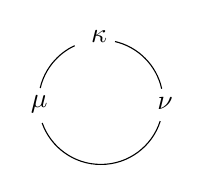
\begin{tikzpicture}[x=0.75pt,y=0.75pt,yscale=-1,xscale=1]
%uncomment if require: \path (0,300); %set diagram left start at 0, and has height of 300

%Shape: Arc [id:dp8573329338560272] 
\draw  [draw opacity=0] (98.78,133.18) .. controls (100.89,124.11) and (107.11,116.62) .. (115.38,112.78) -- (128,140) -- cycle ; \draw   (98.78,133.18) .. controls (100.89,124.11) and (107.11,116.62) .. (115.38,112.78) ;  
%Shape: Arc [id:dp09032135315352707] 
\draw  [draw opacity=0] (156.58,149.13) .. controls (152.72,161.24) and (141.38,170) .. (128,170) .. controls (114.94,170) and (103.83,161.66) .. (99.71,150.01) -- (128,140) -- cycle ; \draw   (156.58,149.13) .. controls (152.72,161.24) and (141.38,170) .. (128,170) .. controls (114.94,170) and (103.83,161.66) .. (99.71,150.01) ;  
%Shape: Arc [id:dp4551353421492913] 
\draw  [draw opacity=0] (134.82,110.78) .. controls (146.02,113.38) and (154.82,122.26) .. (157.3,133.52) -- (128,140) -- cycle ; \draw   (134.82,110.78) .. controls (146.02,113.38) and (154.82,122.26) .. (157.3,133.52) ;  

% Text Node
\draw (93,135.37) node [anchor=north west][inner sep=0.75pt]    {$\mu $};
% Text Node
\draw (154,136.37) node [anchor=north west][inner sep=0.75pt]    {$\nu $};
% Text Node
\draw (122,104.37) node [anchor=north west][inner sep=0.75pt]    {$\kappa $};


\end{tikzpicture}
\end{figure}
\noindent
We now use a cyclic permutation of $\mu, \kappa, \nu $ to obtain the following two equations\footnote{$\lambda$ is summed over in the expression, so we do not consider it in permutation}:
\begin{align*}
    \tensor{\Gamma}{^\lambda _{ \mu \nu}}g_{\kappa \lambda} +\tensor{\Gamma}{^\lambda _{\kappa \nu }}g_{\lambda \mu} &= \partial_\nu g_{\mu\kappa}\\
    \tensor{\Gamma}{^\lambda _{\nu \kappa }}g_{\lambda\mu} +\tensor{\Gamma}{^\lambda _{ \mu \kappa}}g_{\lambda \nu} &= \partial_\kappa g_{\nu\mu}
\end{align*}
Let us now add the first and last equations and subtract the middle one:

\begin{align*}
\partial_\kappa g_{\nu\mu}+\partial_\mu g_{\kappa\nu}- \partial_\nu g_{\mu\kappa}=    \cancel{ \mathcolor{red}{\tensor{\Gamma}{^\lambda _{\nu \kappa }}g_{\lambda\mu}}} +\tensor{\Gamma}{^\lambda _{ \mu \kappa}}g_{\lambda\nu} +\tensor{\Gamma}{^\lambda _{\kappa \mu}}g_{\lambda\nu} +\mathcolor{OliveGreen}{\cancel{\tensor{\Gamma}{^\lambda _{\nu \mu}}g_{\lambda \kappa}}-\cancel{\tensor{\Gamma}{^\lambda _{ \mu \nu}}g_{\lambda\kappa}}} -\cancel{\mathcolor{red}{\tensor{\Gamma}{^\lambda _{\kappa \nu }}g_{\lambda\mu}}}
\end{align*}
We had assumed a torsion-free space and hence the affine connections commute in their lower indices. Hence those terms get cancelled and we finally have the expression as: 
$$\tensor{\Gamma}{^\lambda _{ \mu \kappa}}g_{\lambda\nu} = \frac{1}{2}\brac{\partial_\kappa g_{\nu\mu}+\partial_\mu g_{\kappa\nu}- \partial_\nu g_{\mu\kappa}}$$
Multiply the above by $g^{\nu\alpha}$, then we have: 
\begin{align*}
&\tensor{\Gamma}{^\lambda _{ \mu \kappa}}g_{\lambda\nu} = \frac{1}{2}\brac{\partial_\kappa g_{\nu\mu}+\partial_\mu g_{\kappa\nu}- \partial_\nu g_{\mu\kappa}}\\
\implies &\tensor{\Gamma}{^\lambda _{ \mu \kappa}}g_{\lambda\nu}g^{\nu\alpha} = \frac{1}{2}g^{\nu\alpha}\brac{\partial_\kappa g_{\nu\mu}+\partial_\mu g_{\kappa\nu}- \partial_\nu g_{\mu\kappa}}\\
\implies &\tensor{\Gamma}{^\lambda _{ \mu \kappa}}\tensor{\delta}{^\alpha _\lambda} = \frac{1}{2}g^{\nu\alpha}\brac{\partial_\kappa g_{\nu\mu}+\partial_\mu g_{\kappa\nu}- \partial_\nu g_{\mu\kappa}}\\
\implies &\tensor{\Gamma}{^\alpha _{ \mu \kappa}} = \frac{1}{2}g^{\nu\alpha}\brac{\partial_\kappa g_{\nu\mu}+\partial_\mu g_{\kappa\nu}- \partial_\nu g_{\mu\kappa}}
\end{align*}
Whew!!\emoji{relieved-face} Let us now see an example to find the connection coefficient for 2D polar coordinates.The metric and inverse metric tensor are: 
$$g_{ij} \equiv \begin{pmatrix}
    1 & 0 \\
    0 & r^2
\end{pmatrix}\quad \quad   g^{ij} \equiv \begin{pmatrix}
    1 & 0 \\
    0 & \frac{1}{r^2}
\end{pmatrix}$$
Then taking the derivative of the metric tensor, we have: 
$$\partial_r g_{ij} \equiv \begin{pmatrix}
    1 & 0 \\
    0 & 2r
\end{pmatrix}\quad \quad   \partial_\theta g_{ij} \equiv \begin{pmatrix}
    0 & 0 \\
    0 & 0
\end{pmatrix}$$
The only non-zero element is at $\partial_r g_{\theta \theta}$. Then we only have two non-zero connection coefficients:
\begin{minipage}[t]{0.48\textwidth}
\begin{align*}
\tensor{\Gamma}{^\theta _{r\theta}} &= \frac{1}{2}g^{\theta \theta}\left(\cancel{\partial_\theta g_{\theta r}} + \partial_r g_{\theta \theta} - \cancel{\partial_\theta g_{r \theta}}\right) \\
&= \frac{1}{2r^2} \cdot 2r \\
&= \frac{1}{r}
\end{align*}
\end{minipage}
\hfill
\begin{minipage}[t]{0.48\textwidth}
\begin{align*}
\tensor{\Gamma}{^r _{\theta \theta}} &= \frac{1}{2}g^{r r}\left(\cancel{\partial_\theta g_{r \theta}} + \cancel{\partial_\theta g_{\theta r}} - \partial_r g_{\theta \theta}\right) \\
&= -\frac{1}{2} \cdot 2r \\
&= -r
\end{align*}
\end{minipage}
\subsection{Curls, divergences and other craps}
\subsubsection{Covariant Divergence}

The `ordinary' gradient that we had written earlier, will be generalised to the covariant derivative. Then we will have the divergence modified as: 
\begin{align*}
    \nabla \cdot \tilde{A}\quad \rightarrow \quad \tensor{A}{^\mu _{; \mu}} = \partial_\mu A^\mu + \tensor{\Gamma}{^\mu _{\mu \lambda}}
\end{align*}
From the above relation between metric tensor and the Christoffel symbol, we have:
\begin{align*}
    \tensor{\Gamma}{^\mu _{\mu \lambda}} = \frac{1}{2}g^{\nu \mu}\brac{\partial_\lambda g_{\nu \mu}+\partial_\mu g_{\lambda \nu}-\partial_\nu g_{\mu \lambda}} = \frac{1}{2}\brac{{g^{\nu \mu}\partial_\lambda g_{\nu \mu}}+\mathcolor{blue}{g^{\nu \mu}\partial_\mu g_{\lambda \nu}}-\mathcolor{red}{g^{\nu \mu}\partial_\nu g_{\mu \lambda}}}
\end{align*}
Notice the two coloured terms. Since $\mu$ and $\nu$ are being summed over, we can just interchange them in the, say, red term. Then we will have that both the terms cancel. Thus, we have a simplified expression for the contracted Christoffel symbol as $\tensor{\Gamma}{^\mu _{\mu \lambda}} = \frac{1}{2}g^{\nu \mu}\brac{\partial_\lambda g_{\nu \mu}}$. We will now show that this expression can be reduced to the expression:
$$\tensor{\Gamma}{^\mu _{\mu \lambda}} = \frac{1}{\sqrt{|g|}}\partial_\lambda \brac{\sqrt{|g|}}$$
% $$\tensor{A}{}$$
For that we prove some basic identities:
\begin{identity}
    For any (diagonalisable) matrix $M$, we have:
    $$\Tr (M^{-1}\partial_\lambda M) = \partial_\lambda \ln |M|$$
\end{identity}
\textit{Proof}. Let us calculate the variation of the quantity in the right hand side due to some variation $\delta x^\lambda$ in $x^\lambda$:
\begin{align*}
    \delta \ln |M| &= \ln |M+\delta M| - \ln |M| \\
    &= \ln \brac{\frac{|M+\delta M|}{|M|}} \\
    &= \ln \brac{|M^{-1}||M+\delta M|}\\
    &=\ln \brac{|M^{-1}M + M^{-1}\delta M|}\\
    &=\ln \brac{|\mathds{1}+  M^{-1}\delta M|}
\end{align*}
We now prove another small identity:
$$\ln |M| = \Tr \ln (M)$$
Since M is diagonalisable, we can write the following and then proceed:
\begin{align*}
M &= P D P^{-1}  \\
\Rightarrow \det M &= \det(P D P^{-1}) = \det(D) = \prod_i \lambda_i \\
\Rightarrow \ln \det M &= \ln \left( \prod_i \lambda_i \right) = \sum_i \ln \lambda_i \\
&= \Tr \left( \begin{bmatrix}
\ln \lambda_1 & & \\
& \ln \lambda_2 & \\
& & \ddots
\end{bmatrix} \right) \\
&= \Tr(P^{-1} P \begin{bmatrix}
\ln \lambda_1 & & \\
& \ln \lambda_2 & \\
& & \ddots
\end{bmatrix}) \\
&= \Tr(P \begin{bmatrix}
\ln \lambda_1 & & \\
& \ln \lambda_2 & \\
& & \ddots
\end{bmatrix} P^{-1}) \\
&= \Tr(\ln M)
\end{align*}
So using this identity in the previous result, we have:
\begin{align*}
    \ln \brac{|\mathds{1}+  M^{-1}\delta M|} &= \Tr\ln (\mathds{1}+  M^{-1}\delta M)\\
    &= \Tr\brac{M^{-1}\delta M - \frac{1}{2}{(M^{-1})(\delta M)(M^{-1})(\delta M)}+\ldots}\\
    &=  \Tr M^{-1}\times \delta M  + \ldots
\end{align*}
We somewhat proved this identity\footnote{This derivation is given in Weinberg's book of Cosmology and Gravitation}. Now, we take the case when $M= g$, then we get:
\begin{align*}
   \partial_\lambda \ln |g| =  \Tr(g^{-1}\partial_\lambda g) =\tensor{{\brac{g^{-1}\partial_\lambda g}}}{^\rho _\rho}= \tensor{{g}}{^\rho ^\sigma}\partial_\lambda \tensor{g}{_\sigma _\rho}=2\tensor{\Gamma}{^\mu _\mu _\lambda}
\end{align*}
Thus we get:
$$\tensor{\Gamma}{^\mu _\mu _\lambda} = \frac{1}{2}\partial_\lambda \ln |g|= \frac{1}{2|g|}\partial_\lambda |g|= \frac{1}{\sqrt{|g|}}\partial_\lambda \brac{\sqrt{|g|}}$$
Then we have a cute expression for the covariant divergence:
$$\tensor{A}{^\mu _{; \mu}} = \partial_\mu A^\mu + \frac{1}{\sqrt{|g|}}\partial_\lambda \brac{\sqrt{|g|}}A^\lambda$$
We are not done yet, we can make it even cuter...using the product rule, we have:
$$\partial_\lambda (\sqrt{|g|}A^\lambda) =\sqrt{|g|} \partial_\lambda (A^\lambda)+ \partial_\lambda (\sqrt{|g|}) $$
Substituting this in the above expression, we get: 
$$\tensor{A}{^\mu _{; \mu}} =  \frac{1}{\sqrt{|g|}}\partial_\mu \brac{\sqrt{|g|}A^\mu}$$
Let us check for the spherical polar coordinates where we had seen $g \equiv \mathrm{diag}(1, r^2, r^2\sin\theta) \implies \sqrt{|g|} = r^2 \sin\theta$. Then we will have:
\begin{align*}
    \tensor{A}{^\mu _{; \mu}} &= \frac{1}{r^2 \sin\theta}\brac{\pdv{(r^2\sin\theta A^1)}{r}+\pdv{(r^2\sin\theta A^2)}{\theta}+\pdv{(r^2\sin\theta A^3)}{\phi}}\\
    &=\frac{1}{r^2 \sin\theta}\brac{\sin\theta \pdv{(A^1r^2)}{r}+r^2\pdv{(A^2\sin\theta )}{\theta}+r^2\sin\theta\pdv{( A^3)}{\phi}}\\
   &= {\frac{1}{r^2} \pdv{(A^1r^2)}{r}+\frac{1}{\sin\theta}\pdv{(A^2\sin\theta )}{\theta}+\pdv{( A^3)}{\phi}}
\end{align*}
Now, note that we had earlier done said something about ordinary vectors and how they relate to contravariant vector: $A^\mu = \frac{\widetilde{A_\mu}}{h_\mu}$ and we had also seen the relation between them in spherical coordinates. Using that we have:
\begin{align*}
    \tensor{A}{^\mu _{; \mu}} &= {\frac{1}{r^2} \pdv{(\widetilde{A}_r r^2)}{r}+\frac{1}{\sin\theta}\pdv{(\frac{\widetilde{A}_\theta}{r}\sin\theta )}{\theta}+\pdv{(\frac{\widetilde{A}_\phi}{r\sin\theta})}{\phi}}\\
    &={\frac{1}{r^2} \pdv{(\widetilde{A}_r r^2)}{r}+\frac{1}{r\sin\theta}\pdv{({\widetilde{A}_\theta}\sin\theta )}{\theta}+\frac{1}{{r\sin\theta}}\pdv{({\widetilde{A}_\phi})}{\phi}}
\end{align*}
Lol, this is the formula for normal divergence in spherical polar coordinates that we had been studying and so this new `cute' formula makes sense! Let us now check for the Laplacian and curl too. 
\subsubsection{Covariant Laplacian}
We calculate the following \footnote{Note that the components of the covariant derivative of a scalar function are just the partial derivatives} for a scalar function $\upphi$:
\begin{align*}
    D_\mu D^\mu \upphi = \frac{1}{\sqrt{|g|}}\partial_\mu \brac{\sqrt{|g|}\partial^\mu \upphi}
\end{align*}
Well, note that $\partial^\mu \upphi = g^{\mu \nu}\partial_\nu$ and since the metric tensor is diagonal in this case, only $g^{rr}=1, g^{\theta\theta}=\frac{1}{r^2}, g^{\phi\phi} = \frac{1}{r^2\sin^2\theta}$ will contribute. We then substitute it in the above:
\begin{align*}
    \frac{1}{\sqrt{|g|}} \partial_\mu \left( \sqrt{|g|} \partial^\mu \upphi \right)
    &= \frac{1}{\sqrt{|g|}} \partial_\mu \left( \sqrt{|g|} g^{\mu \nu} \partial_\nu \upphi \right) \\
    &= \frac{1}{r^2 \sin\theta} 
       \brac{ \pdv{}{r} \left( r^2 \sin\theta \pdv{\upphi}{r} \right)
        + \pdv{}{\theta} \left( r^2 \sin\theta \frac{1}{r^2}\cdot\pdv{\upphi}{\theta} \right)
        + \pdv{}{\phi} \left( r^2  \frac{1}{r^2\sin^2\theta}\cdot\pdv{\upphi}{\phi} \right)}\\
    &=\frac{1}{r^2} \pdv{}{r} \left( r^2  \pdv{\upphi}{r} \right) + \frac{1}{r^2\sin\theta}\pdv{}{\theta} \left(  \sin\theta \pdv{\upphi}{\theta} \right) + \frac{1}{r^2\sin^2\theta}\pdv[2]{\upphi}{\phi}
\end{align*}
Wasn't this nice and simple, to derive the form of the Laplacian which has scared us for so long because it just looked ghastly and seemingly popped out of nowhere? 
\subsubsection{A Thing or Two about Levi-Civita}
Curls and cross-products cannot be done without the mention of Levi-Civita symbol. So, let us see a few things about that thing first. 
We all know the famous $\upepsilon_{ijk}$, let us generalise this to higher number of indices and write it with a tilde. So, what we have is:
$$\widetilde{\upepsilon}_{\mu_1\mu_2\ldots\mu_n} = \begin{cases}
    +1, \text{If } {\mu_1\mu_2\ldots\mu_n} \text{is even permutation of } \{0,1,2,\ldots, (n-1)\} \\
     -1, \text{If } {\mu_1\mu_2\ldots\mu_n} \text{is odd permutation of } \{0,1,2,\ldots, (n-1)\}\\
     +0, \text{otherwise}
\end{cases}$$
We will call this object the Levi-Civita `symbol', specifically, since this is not a tensor. Now note one identity:
\begin{identity}
$$\widetilde{\upepsilon}_{\mu_1'\ldots \mu_n'}\det(M)= \widetilde{\upepsilon}_{\mu_1\ldots \mu_n} \tensor{M}{^{\mu_1} _{\mu_1'}}\tensor{M}{^{\mu_2} _{\mu_2'}}\ldots\tensor{M}{^{\mu_n} _{\mu_n'}}$$
\end{identity}
Now take the matrix $M \equiv \pdv{x}{x'}$, then we have from the above formula:
$$\widetilde{\upepsilon}_{\mu_1'\ldots \mu_n'}\left|\pdv{x}{x'}\right|= \widetilde{\upepsilon}_{\mu_1\ldots \mu_n} \pdv{x^{\mu_1}}{x_{\mu_1'}}\pdv{x^{\mu_2}}{x_{\mu_2'}}\ldots\pdv{x^{\mu_n}}{x_{\mu_n'}}\implies\widetilde{\upepsilon}_{\mu_1'\ldots \mu_n'}=\left|\pdv{x'}{x}\right| \widetilde{\upepsilon}_{\mu_1\ldots \mu_n} \pdv{x^{\mu_1}}{x_{\mu_1'}}\pdv{x^{\mu_2}}{x_{\mu_2'}}\ldots\pdv{x^{\mu_n}}{x_{\mu_n'}} $$
We just took the determinant in the denominator in the right hand side and then took the inverse matrix, since inverse of the determinant of a matrix is the determinant of its inverse. \footnote{By the way, I really like these kind of reciprocal sentences. It's a cool thing about mathematics! Another example may be, like sum of trace is the trace of sum.}However, note that the matrix is just the Jacobian and hence the Levi-Civita symbol is a \textit{tensor density} of weight $+1$. Now, also remember that we had previously seen:
$$\mathrm{J} = \sqrt{\frac{|g|}{|g'|}}$$
Then, we will have:
$$\widetilde{\upepsilon}_{\mu_1'\ldots \mu_n'}= \sqrt{\frac{|g|}{|g'|}} \widetilde{\upepsilon}_{\mu_1\ldots \mu_n} \pdv{x^{\mu_1}}{x_{\mu_1'}}\pdv{x^{\mu_2}}{x_{\mu_2'}}\ldots\pdv{x^{\mu_n}}{x_{\mu_n'}}\implies \sqrt{{|g'|}}\widetilde{\upepsilon}_{\mu_1'\ldots \mu_n'}= \sqrt{{|g|}} \widetilde{\upepsilon}_{\mu_1\ldots \mu_n} \pdv{x^{\mu_1}}{x_{\mu_1'}}\pdv{x^{\mu_2}}{x_{\mu_2'}}\ldots\pdv{x^{\mu_n}}{x_{\mu_n'}} $$
Thus the quantity ${\upepsilon}_{\mu_1\ldots\mu_n} = \sqrt{|g|}\widetilde{\upepsilon}_{\mu_1\ldots\mu_n}$ transforms as a tensor and we can do all the up and down game with the indices. This we call as \textbf{Levi-Civita tensor}. We also sometimes define the Levi-Civita symbol as $\widetilde{\upepsilon}^{\mu_1'\ldots \mu_n'}$ which is of weight $-1$\footnote{This is numerically equal to $\mathrm{sgn}(g) \widetilde{\upepsilon}_{\mu_1\ldots\mu_n}$} and then we get ${\upepsilon}^{\mu_1\ldots\mu_n} = \frac{1}{\sqrt{|g|}}\widetilde{\upepsilon}^{\mu_1\ldots\mu_n}$.\\[0.3cm]
Most of the time, we contract some of the indices of the Levi-Civita tensor and we obtain some Kronecker deltas. We have an identity for contracting $p$ such indices: 
$$\epsilon^{\mu_1 \mu_2 \cdots \mu_p \alpha_1 \cdots \alpha_{n-p}} 
\epsilon_{\mu_1 \mu_2 \cdots \mu_p \beta_1 \cdots \beta_{n-p}} 
= (-1)^s\, p!(n - p)! \, \delta^{[\alpha_1\ldots \alpha_{n-p}]}_{\beta_1\ldots \beta_{n-p}}$$
Now, wtf does the right hand side denote? Here $s$ is the number of negative eigenvalues of the metric tensor but what about the weird delta symbol? Carroll writes it as an anti-symmetrised product of Kronecker deltas. We elaborate it a bit further. For any tensor $T$, the notation $\tensor{T}{^{[\mu_1\ldots\mu_n]}}$ is equal to: 
$$\tensor{T}{^{[\mu_1\ldots\mu_n]}} = \frac{1}{n!}\sum\limits_{\pi \in S_n}\mathrm{sgn}(\pi)\tensor{T}{^{\mu_{\pi(1)}\mu_{\pi(2)}\ldots\mu_{\pi(n)}}}$$
Well, did I make it more complicated? Perhaps, but complications lead to clarifications. $S_n$ is the permutation group of order $n$, $\mathrm{sgn}(\pi)$ denotes the sign of the permutation and is positive if it is obtained from even number of exchanges and negative otherwise. Let us see for $S_3$, the group is then:
$$S_3\equiv  \{\underbrace{\{1,2,3\}}_{\pi_1},\underbrace{\{1,3,2\}}_{\pi_2},\underbrace{\{2,1,3\}}_{\pi_3},\underbrace{\{2,3,1\}}_{\pi_4},\underbrace{\{3,1,2\}}_{\pi_5},\underbrace{\{3,2,1\}}_{\pi_6} \}$$
Then we can check that we have $\mathrm{sgn}(\pi_i) = +1$ for $i=1,4,5$ and $-1$ for $i=2,3,6$
So, similarly the Kronecker delta can be written as: 
$$\tensor{\delta}{^{[\alpha_1\ldots\alpha_{n-p}]} _{\beta_1\ldots\beta_{n-p}}} = \frac{1}{(n-p)!}\sum\limits_{\pi \in S_n}\mathrm{sgn}(\pi) \prod\limits_i \tensor{\delta}{^{\alpha_{\pi(i)}} _{\beta(i)}}$$
And now using Leibniz's formula for determinant\footnote{The formula says that for any matrix A, we have:
$$\det(A) = \sum_{\tau \in S_n} \operatorname{sgn}(\tau) \prod_{i=1}^{n} a^{i}_{\tau(i)} 
= \sum_{\sigma \in S_n} \operatorname{sgn}(\sigma) \prod_{i=1}^{n} a_{\sigma(i)}^{i}$$
}, we have: 
$$\tensor{\delta}{^{[\alpha_1\ldots\alpha_{n-p}]} _{\beta_1\ldots\beta_{n-p}}} = \frac{1}{(n-p)!}\det(\mathrm{\delta})$$
where, $$\delta \equiv 
\begin{pmatrix}
\delta^{\alpha_1}_{\beta_1} & \cdots & \delta^{\alpha_{n-p}}_{\beta_1} \\
\vdots & \ddots & \vdots \\
\delta^{\alpha_1}_{\beta_{n-p}} & \cdots & \delta^{\alpha_{n-p}}_{\beta_{n-p}}
\end{pmatrix}$$
Then the final expression that we have is: 
$$\epsilon^{\mu_1 \mu_2 \cdots \mu_p \alpha_1 \cdots \alpha_{n-p}} 
\epsilon_{\mu_1 \mu_2 \cdots \mu_p \beta_1 \cdots \beta_{n-p}} 
= (-1)^s p! \det{\delta}$$
Well, let us see one example, for this that we know. For this, we take $p=1$ and $n=3$, then $n-p = 2$. So, we have:
$$\epsilon^{ijk}\epsilon{ilm} = (-1)^s \times 1! \times \det\begin{pmatrix}
    \delta^j_l &  \delta^k_l \\
     \delta^j_m &  \delta^k_m
\end{pmatrix} = (-1)^s \brac{\delta^j_l \delta^k_m - \delta^j_m \delta^k_l}$$
Isn't this fun to finally see how this expression comes? Well, for me, yes but it is just an amusement for me, 'coz ultimately, to use it, we have to kinda remember it. Deriving things from scratch is a painful patch, with time to lose and little to match. 
\subsubsection{Covariant Curl}




\section{Bit of  Differential Geometry: Dayuum!!}
Let us look into a bit of differential geometry which is a formal way of treating this tensor thingy. We will try to be as intuitive and non-rigorous as possible (and thus increasing our chances of making a mathematician crazy!) but yeah, we will try to be rigorous enough so that I am satisfied.
\subsection{Some prior things}
Before touching manifolds, let us define what an abstract topological space is, since manifolds are special case of topological spaces. 
\begin{definition}[Topological Space]
  A topological space is a set $(X, \uptau )$ where $\uptau \subset \mathcal{P}$ is a collection of subsets of $X$ such that:
\begin{itemize}
    \item $\emptyset, X \in \uptau$.
    \item $U_\alpha \in \uptau \implies \bigcup \limits_{\alpha\in J} U_\alpha \in \uptau$  (closed under arbitrary union).
    \item $U_i \in \uptau \implies \bigcap \limits_{i=1}^n U_i \in \uptau$  (closed under finite intersection)\footnotemark.
\end{itemize}
\end{definition}
\footnote{Here $\alpha$ index is used when we want the indexing set $J$ (indexing set means the set from where the incides to denote the elements of the set are taken from) to be arbitrary, meaning that the set $\{U_\alpha\}$ can be finite, countable or uncountable. On the other hand, index $i$ is mostly used when the indexing set is finite.}

Well well, this does not look anything like coffee cup and donut which most people associate topology with. That is a case of \textit{homeomorphism} which will be discussed later (hopefully). However, for now let us proceed. The sets belonging to $\uptau$ are called \textbf{open sets}. We define a \textbf{closed set} as a set whose complement is open. There are umpteen other definitions like \textbf{closure, boundary, interior, neighbourhood}, etc. Let define few of them \emoji{loudly-crying-face}. 
\begin{itemize}
    \item \textit{Closure} of a set $A$ is the smallest closed set containing $A$ and is denoted by $\overline{A}$.
    \item \textit{Interior} of a set $A$ is the largest open set contained in $A$ and is denoted by $\text{int}(A)$.
    \item \textit{Boundary} of a set $A$ is the set of points which are neither in the interior nor in the exterior of $A$ and is denoted by $\partial A$.
    \item If $p\in X$, then a \textit{neighbourhood} of $p$ is a set $N$ such that there exists an open set $U\in \uptau$ with $p\in U\subseteq N$.
\begin{figure}[H]
      \centering
      

\tikzset{every picture/.style={line width=0.75pt}} %set default line width to 0.75pt        

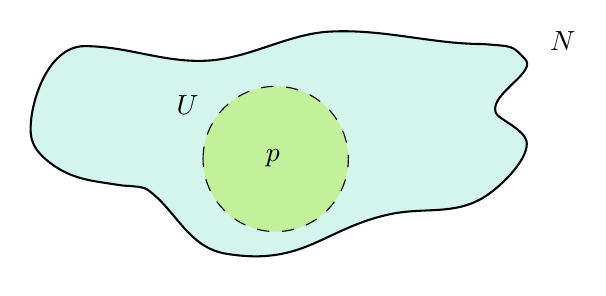
\begin{tikzpicture}[x=0.75pt,y=0.75pt,yscale=-1,xscale=1]
%uncomment if require: \path (0,203); %set diagram left start at 0, and has height of 203

%Curve Lines [id:da28281619681811754] 
\draw [fill={rgb, 255:red, 211; green, 245; blue, 236 }  ,fill opacity=1 ][line width=0.75] [line join = round][line cap = round]   (264,41.63) .. controls (239.07,41.63) and (216.02,34.24) .. (190,35.63) .. controls (169.94,36.71) and (151.25,48.57) .. (131,49.63) .. controls (109.98,50.74) and (92.57,42.63) .. (72,42.63) .. controls (53.59,42.63) and (45.01,71.73) .. (46,84.63) .. controls (46.47,90.7) and (50.18,94.88) .. (55,98.63) .. controls (66.08,107.25) and (76.24,107.51) .. (89,109.63) .. controls (91.95,110.13) and (99.58,109.96) .. (102,111.63) .. controls (115.88,121.24) and (121.56,139.56) .. (140,142.63) .. controls (177.55,148.89) and (187.14,130.46) .. (219,123.63) .. controls (235.52,120.09) and (249.69,124.22) .. (264,115.63) .. controls (271.71,111.01) and (285,98.32) .. (285,89.63) .. controls (285,82.9) and (271.1,77.94) .. (270,74.63) .. controls (266.91,65.36) and (290.59,55.22) .. (284,48.63) .. controls (277.54,42.17) and (279,42.85) .. (264,41.63) -- cycle ;
%Shape: Circle [id:dp001327175657310109] 
\draw  [fill={rgb, 255:red, 194; green, 241; blue, 156 }  ,fill opacity=1 ][dash pattern={on 4.5pt off 4.5pt}] (129,97) .. controls (129,77.67) and (144.67,62) .. (164,62) .. controls (183.33,62) and (199,77.67) .. (199,97) .. controls (199,116.33) and (183.33,132) .. (164,132) .. controls (144.67,132) and (129,116.33) .. (129,97) -- cycle ;

% Text Node
\draw (158,91.4) node [anchor=north west][inner sep=0.75pt]    {$p$};
% Text Node
\draw (115,65.4) node [anchor=north west][inner sep=0.75pt]    {$U$};
% Text Node
\draw (295,34.4) node [anchor=north west][inner sep=0.75pt]    {$N$};


\end{tikzpicture}

      \caption{Neighbourhood of a point $p$ in  $X$}
\end{figure}
          \item \textit{Hausdorff Space}: A topological space is called Hausdorff if for any two distinct points $x,y\in X$, there exist open sets $U,V\in \uptau$ such that $x\in U, y\in V$ and $U\cap V = \emptyset$. 
    \begin{figure}[H]
      \centering
      

\tikzset{every picture/.style={line width=0.75pt}} %set default line width to 0.75pt        

\begin{tikzpicture}[x=0.75pt,y=0.75pt,yscale=-1,xscale=1]
%uncomment if require: \path (0,203); %set diagram left start at 0, and has height of 203

%Shape: Circle [id:dp44753041237162206] 
\draw  [dash pattern={on 4.5pt off 4.5pt}] (129,97) .. controls (129,77.67) and (144.67,62) .. (164,62) .. controls (183.33,62) and (199,77.67) .. (199,97) .. controls (199,116.33) and (183.33,132) .. (164,132) .. controls (144.67,132) and (129,116.33) .. (129,97) -- cycle ;
%Shape: Circle [id:dp09577026242923825] 
\draw  [dash pattern={on 4.5pt off 4.5pt}] (230,98.5) .. controls (230,75.03) and (249.03,56) .. (272.5,56) .. controls (295.97,56) and (315,75.03) .. (315,98.5) .. controls (315,121.97) and (295.97,141) .. (272.5,141) .. controls (249.03,141) and (230,121.97) .. (230,98.5) -- cycle ;

% Text Node
\draw (159,92.4) node [anchor=north west][inner sep=0.75pt]    {$x$};
% Text Node
\draw (267,92.4) node [anchor=north west][inner sep=0.75pt]    {$y$};
% Text Node
\draw (113,56.4) node [anchor=north west][inner sep=0.75pt]    {$U$};
% Text Node
\draw (307,47.4) node [anchor=north west][inner sep=0.75pt]    {$V$};


\end{tikzpicture}

      \caption{A \textbf{Hausdorff Space}, where the points $x$ and $y$ are separated by the open sets $U$ and $V$.}
    \end{figure}
    \item \textit{Topological Continuity}: A function $f: X \to Y$ between two topological spaces is said to be continuous if for every open set $V \in \uptau_Y$, the preimage $f^{-1}(V)\footnote{The preimage of a set $Y$ under the function $f$ is defined as $f^{-1}(Y) = \{x|f(x)\in Y\}$. Note that this has nothing to do with inverse of a function (sadly we use the same notation)} \in \uptau_X$ is open in $X$.
    \item \textit{Homeomorphism}: A homeomorphism is a bijective function $f: X\to Y$ between two topological spaces such that both $f$ and its inverse $f^{-1}$ are continuous. If such a function exists, we say that the two spaces are \textbf{homeomorphic} and we write $X\cong Y$.
    \item \textit{Cover:} A cover of a topological space $X$ is a collection of sets $\{U_\alpha \}$whose union is $X$ that is, $\bigcup\limits_\alpha U_\alpha = X$. If each set is an open set, then it is called an \textbf{open cover}. If there exists a finite collection of subsets of the cover such that their union is $X$, that is, $\bigcup\limits_{i=1}^k U_i = X$ then it is called a \textbf{finite subcover}.
    \begin{figure}[H]
    \centering
    

\tikzset{every picture/.style={line width=0.75pt}} %set default line width to 0.75pt        

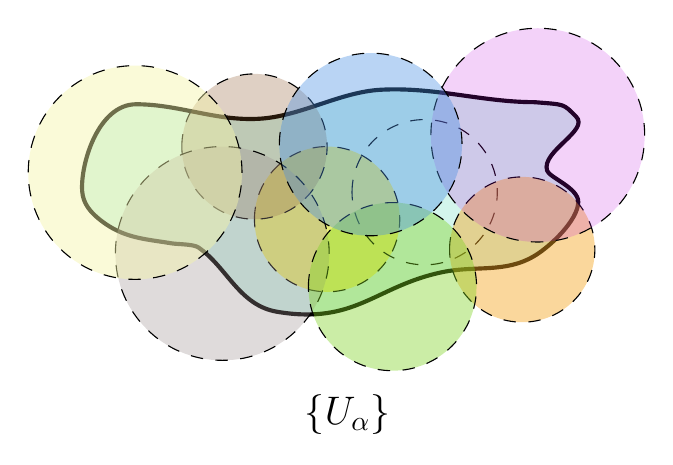
\begin{tikzpicture}[x=0.75pt,y=0.75pt,yscale=-1,xscale=1]
%uncomment if require: \path (0,227); %set diagram left start at 0, and has height of 227

%Curve Lines [id:da28281619681811754] 
\draw [fill={rgb, 255:red, 211; green, 245; blue, 236 }  ,fill opacity=1 ][line width=1.5] [line join = round][line cap = round]   (264,40.63) .. controls (239.07,40.63) and (216.02,33.24) .. (190,34.63) .. controls (169.94,35.71) and (151.25,47.57) .. (131,48.63) .. controls (109.98,49.74) and (92.57,41.63) .. (72,41.63) .. controls (53.59,41.63) and (45.01,70.73) .. (46,83.63) .. controls (46.47,89.7) and (50.18,93.88) .. (55,97.63) .. controls (66.08,106.25) and (76.24,106.51) .. (89,108.63) .. controls (91.95,109.13) and (99.58,108.96) .. (102,110.63) .. controls (115.88,120.24) and (121.56,138.56) .. (140,141.63) .. controls (177.55,147.89) and (187.14,129.46) .. (219,122.63) .. controls (235.52,119.09) and (249.69,123.22) .. (264,114.63) .. controls (271.71,110.01) and (285,97.32) .. (285,88.63) .. controls (285,81.9) and (271.1,76.94) .. (270,73.63) .. controls (266.91,64.36) and (290.59,54.22) .. (284,47.63) .. controls (277.54,41.17) and (279,41.85) .. (264,40.63) -- cycle ;
%Shape: Circle [id:dp001327175657310109] 
\draw  [fill={rgb, 255:red, 248; green, 231; blue, 28 }  ,fill opacity=0.55 ][dash pattern={on 4.5pt off 4.5pt}] (129,97) .. controls (129,77.67) and (144.67,62) .. (164,62) .. controls (183.33,62) and (199,77.67) .. (199,97) .. controls (199,116.33) and (183.33,132) .. (164,132) .. controls (144.67,132) and (129,116.33) .. (129,97) -- cycle ;
%Shape: Circle [id:dp7871419017635473] 
\draw  [dash pattern={on 4.5pt off 4.5pt}] (176,84) .. controls (176,64.67) and (191.67,49) .. (211,49) .. controls (230.33,49) and (246,64.67) .. (246,84) .. controls (246,103.33) and (230.33,119) .. (211,119) .. controls (191.67,119) and (176,103.33) .. (176,84) -- cycle ;
%Shape: Circle [id:dp8717686595013016] 
\draw  [fill={rgb, 255:red, 245; green, 166; blue, 35 }  ,fill opacity=0.45 ][dash pattern={on 4.5pt off 4.5pt}] (223,111.63) .. controls (223,92.3) and (238.67,76.63) .. (258,76.63) .. controls (277.33,76.63) and (293,92.3) .. (293,111.63) .. controls (293,130.96) and (277.33,146.63) .. (258,146.63) .. controls (238.67,146.63) and (223,130.96) .. (223,111.63) -- cycle ;
%Shape: Circle [id:dp9588061758851951] 
\draw  [fill={rgb, 255:red, 139; green, 87; blue, 42 }  ,fill opacity=0.28 ][dash pattern={on 4.5pt off 4.5pt}] (94,62) .. controls (94,42.67) and (109.67,27) .. (129,27) .. controls (148.33,27) and (164,42.67) .. (164,62) .. controls (164,81.33) and (148.33,97) .. (129,97) .. controls (109.67,97) and (94,81.33) .. (94,62) -- cycle ;
%Shape: Circle [id:dp9449595488988661] 
\draw  [fill={rgb, 255:red, 158; green, 145; blue, 145 }  ,fill opacity=0.33 ][dash pattern={on 4.5pt off 4.5pt}] (62,113.5) .. controls (62,85.06) and (85.06,62) .. (113.5,62) .. controls (141.94,62) and (165,85.06) .. (165,113.5) .. controls (165,141.94) and (141.94,165) .. (113.5,165) .. controls (85.06,165) and (62,141.94) .. (62,113.5) -- cycle ;
%Shape: Circle [id:dp5330131974534975] 
\draw  [fill={rgb, 255:red, 189; green, 16; blue, 224 }  ,fill opacity=0.19 ][dash pattern={on 4.5pt off 4.5pt}] (214,56.5) .. controls (214,28.06) and (237.06,5) .. (265.5,5) .. controls (293.94,5) and (317,28.06) .. (317,56.5) .. controls (317,84.94) and (293.94,108) .. (265.5,108) .. controls (237.06,108) and (214,84.94) .. (214,56.5) -- cycle ;
%Shape: Circle [id:dp4837000860245192] 
\draw  [fill={rgb, 255:red, 126; green, 211; blue, 33 }  ,fill opacity=0.4 ][dash pattern={on 4.5pt off 4.5pt}] (155,129.5) .. controls (155,107.13) and (173.13,89) .. (195.5,89) .. controls (217.87,89) and (236,107.13) .. (236,129.5) .. controls (236,151.87) and (217.87,170) .. (195.5,170) .. controls (173.13,170) and (155,151.87) .. (155,129.5) -- cycle ;
%Shape: Circle [id:dp17768072579265115] 
\draw  [fill={rgb, 255:red, 74; green, 144; blue, 226 }  ,fill opacity=0.39 ][dash pattern={on 4.5pt off 4.5pt}] (141,61) .. controls (141,36.7) and (160.7,17) .. (185,17) .. controls (209.3,17) and (229,36.7) .. (229,61) .. controls (229,85.3) and (209.3,105) .. (185,105) .. controls (160.7,105) and (141,85.3) .. (141,61) -- cycle ;
%Shape: Circle [id:dp406181221930618] 
\draw  [fill={rgb, 255:red, 244; green, 245; blue, 168 }  ,fill opacity=0.45 ][dash pattern={on 4.5pt off 4.5pt}] (20,74.5) .. controls (20,46.06) and (43.06,23) .. (71.5,23) .. controls (99.94,23) and (123,46.06) .. (123,74.5) .. controls (123,102.94) and (99.94,126) .. (71.5,126) .. controls (43.06,126) and (20,102.94) .. (20,74.5) -- cycle ;

% Text Node
\draw (152,180.4) node [anchor=north west][inner sep=0.75pt]  [font=\Large]  {$\{U_{\alpha }\}$};


\end{tikzpicture}

    \caption{Open cover of a space}
  \end{figure}
  \item \textit{Subspace Topology }is the topology on a subset $Y\subseteq X$ induced by the topology of $X$. In this case, open sets of $Y$ are basically the intersection of open sets of $X$ with $Y$. So,
  $$\uptau_Y = \{U\cap Y| U\in \uptau_X\}$$
  \end{itemize}
\subsection{Manifolds}
Let us see some pictures. 
\begin{figure}[H]
  \centering

  \begin{subfigure}[b]{0.3\textwidth}
    \centering
    

\tikzset{every picture/.style={line width=0.75pt}} %set default line width to 0.75pt        

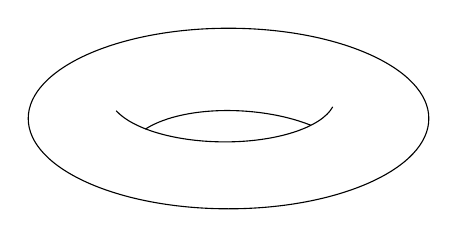
\begin{tikzpicture}[x=0.75pt,y=0.75pt,yscale=-1,xscale=1]
%uncomment if require: \path (0,300); %set diagram left start at 0, and has height of 300

%Shape: Ellipse [id:dp22801969143067424] 
\draw   (104,164.5) .. controls (104,140.48) and (147.2,121) .. (200.5,121) .. controls (253.8,121) and (297,140.48) .. (297,164.5) .. controls (297,188.52) and (253.8,208) .. (200.5,208) .. controls (147.2,208) and (104,188.52) .. (104,164.5) -- cycle ;
%Shape: Arc [id:dp10077529814620967] 
\draw  [draw opacity=0] (250.72,158.87) .. controls (245.28,168.82) and (223.36,176.06) .. (197.24,175.75) .. controls (173.88,175.48) and (154.02,169.25) .. (146.36,160.73) -- (197.5,153.5) -- cycle ; \draw   (250.72,158.87) .. controls (245.28,168.82) and (223.36,176.06) .. (197.24,175.75) .. controls (173.88,175.48) and (154.02,169.25) .. (146.36,160.73) ;  
%Shape: Arc [id:dp345385029103655] 
\draw  [draw opacity=0] (160.45,169.6) .. controls (170.37,163.16) and (188.19,159.59) .. (208.22,160.93) .. controls (220.26,161.74) and (231.27,164.2) .. (240.09,167.72) -- (206.61,184.82) -- cycle ; \draw   (160.45,169.6) .. controls (170.37,163.16) and (188.19,159.59) .. (208.22,160.93) .. controls (220.26,161.74) and (231.27,164.2) .. (240.09,167.72) ;  





\end{tikzpicture}

    \caption{Torus (yeah, donut came atlast!)}
  \end{subfigure}
  \hfill
  \begin{subfigure}[b]{0.3\textwidth}
    \centering
    

\tikzset{every picture/.style={line width=0.75pt}} %set default line width to 0.75pt        

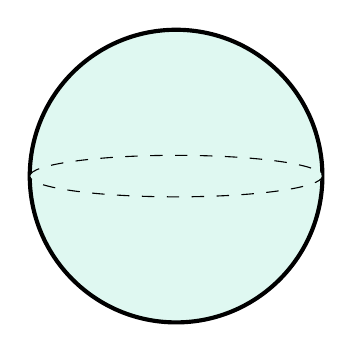
\begin{tikzpicture}[x=0.75pt,y=0.75pt,yscale=-1,xscale=1]
%uncomment if require: \path (0,300); %set diagram left start at 0, and has height of 300

%Shape: Circle [id:dp5828809729635696] 
\draw  [fill={rgb, 255:red, 223; green, 248; blue, 241 }  ,fill opacity=1 ][line width=1.5]  (161,152.5) .. controls (161,113.56) and (192.56,82) .. (231.5,82) .. controls (270.44,82) and (302,113.56) .. (302,152.5) .. controls (302,191.44) and (270.44,223) .. (231.5,223) .. controls (192.56,223) and (161,191.44) .. (161,152.5) -- cycle ;
%Shape: Ellipse [id:dp9903216585683989] 
\draw  [fill={rgb, 255:red, 223; green, 248; blue, 241 }  ,fill opacity=1 ][dash pattern={on 4.5pt off 4.5pt}] (161,152.5) .. controls (161,146.98) and (192.56,142.5) .. (231.5,142.5) .. controls (270.44,142.5) and (302,146.98) .. (302,152.5) .. controls (302,158.02) and (270.44,162.5) .. (231.5,162.5) .. controls (192.56,162.5) and (161,158.02) .. (161,152.5) -- cycle ;




\end{tikzpicture}

    \caption{Sphere (like yo mama)}
  \end{subfigure}
  \hfill
  \begin{subfigure}[b]{0.3\textwidth}
    \centering
    

\tikzset{every picture/.style={line width=0.75pt}} %set default line width to 0.75pt        

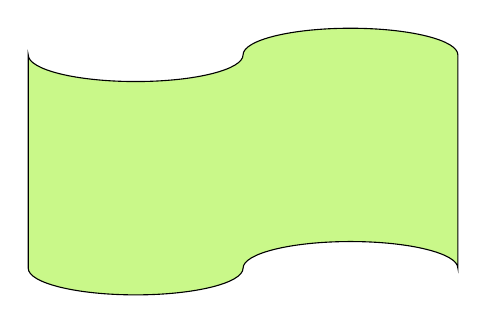
\begin{tikzpicture}[x=0.75pt,y=0.75pt,yscale=-1,xscale=1]
%uncomment if require: \path (0,300); %set diagram left start at 0, and has height of 300

%Flowchart: Punched Tape [id:dp25700721970086793] 
\draw  [fill={rgb, 255:red, 201; green, 248; blue, 137 }  ,fill opacity=1 ] (155,67.85) .. controls (155,74.94) and (178.17,80.69) .. (206.75,80.69) .. controls (235.33,80.69) and (258.5,74.94) .. (258.5,67.85) .. controls (258.5,60.75) and (281.67,55) .. (310.25,55) .. controls (338.83,55) and (362,60.75) .. (362,67.85) -- (362,170.62) .. controls (362,163.52) and (338.83,157.77) .. (310.25,157.77) .. controls (281.67,157.77) and (258.5,163.52) .. (258.5,170.62) .. controls (258.5,177.72) and (235.33,183.47) .. (206.75,183.47) .. controls (178.17,183.47) and (155,177.72) .. (155,170.62) -- cycle ;




\end{tikzpicture}

    \caption{A Waving Flag perhaps?}
  \end{subfigure}

  \caption{\textbf{What's common in all these?}}
\end{figure}
\noindent
So, what is common in all these pictures? Note that they all look very different from each other but if we really ZOOM in \emoji{mag-right} we can see that each of them look alike, like a \textit{flat plane}. Well, the road ahead of us looks flat but the road is on the freaking Earth which is, let's say to a physicist's satisfaction, a sphere. So, we can say that all of these things look `locally' like the flat plane $\mathbb{R}^2$. This is essentially the idea behind a \textbf{manifold}, things which look locally Euclidean (like $\mathbb{R}^n$). Let us define manifolds formally:
\begin{definition}[Manifold]
  $\mathcal{M}$ is a m-dimensional manifold if:
  \begin{itemize}
    \item $\mathcal{M}$ is a topological space.
    \item There exists an open cover $\{U_\alpha\}$ of $\mathcal{M}$ and for each $\alpha$, there exists a homeomorphism $\phi_\alpha: U_\alpha \to V_\alpha$ where $V_\alpha$ is an open subset of $\mathbb{R}^m$.
    \item Two open sets $U_i, U_j$ such that $U_i \cap U_j \neq \emptyset$, then the map $\psi_{ij} = \phi_i \circ \phi_j^{-1}$ is a smooth map \footnotemark, where $\psi_{ij}: \phi_j(U_i \cap U_j) \to \phi_i(U_i \cap U_j)$.
  \end{itemize}
\end{definition}
\footnotetext{
A smooth map is a function which is infinitely differentiable, that is, all the derivatives exist and are continuous. Sometimes a smooth map $f$ is said to belong to the class $C^\infty$. In general, $C^k$ is the class of functions which are $k$ times continuously differentiable. }
\begin{figure}[H]
  \centering 
  

% Pattern Info
 
\tikzset{
pattern size/.store in=\mcSize, 
pattern size = 5pt,
pattern thickness/.store in=\mcThickness, 
pattern thickness = 0.3pt,
pattern radius/.store in=\mcRadius, 
pattern radius = 1pt}
\makeatletter
\pgfutil@ifundefined{pgf@pattern@name@_z2kbg8xsc}{
\pgfdeclarepatternformonly[\mcThickness,\mcSize]{_z2kbg8xsc}
{\pgfqpoint{0pt}{0pt}}
{\pgfpoint{\mcSize+\mcThickness}{\mcSize+\mcThickness}}
{\pgfpoint{\mcSize}{\mcSize}}
{
\pgfsetcolor{\tikz@pattern@color}
\pgfsetlinewidth{\mcThickness}
\pgfpathmoveto{\pgfqpoint{0pt}{0pt}}
\pgfpathlineto{\pgfpoint{\mcSize+\mcThickness}{\mcSize+\mcThickness}}
\pgfusepath{stroke}
}}
\makeatother

% Pattern Info
 
\tikzset{
pattern size/.store in=\mcSize, 
pattern size = 5pt,
pattern thickness/.store in=\mcThickness, 
pattern thickness = 0.3pt,
pattern radius/.store in=\mcRadius, 
pattern radius = 1pt}
\makeatletter
\pgfutil@ifundefined{pgf@pattern@name@_gl41bao2a}{
\pgfdeclarepatternformonly[\mcThickness,\mcSize]{_gl41bao2a}
{\pgfqpoint{0pt}{0pt}}
{\pgfpoint{\mcSize+\mcThickness}{\mcSize+\mcThickness}}
{\pgfpoint{\mcSize}{\mcSize}}
{
\pgfsetcolor{\tikz@pattern@color}
\pgfsetlinewidth{\mcThickness}
\pgfpathmoveto{\pgfqpoint{0pt}{0pt}}
\pgfpathlineto{\pgfpoint{\mcSize+\mcThickness}{\mcSize+\mcThickness}}
\pgfusepath{stroke}
}}
\makeatother

% Pattern Info
 
\tikzset{
pattern size/.store in=\mcSize, 
pattern size = 5pt,
pattern thickness/.store in=\mcThickness, 
pattern thickness = 0.3pt,
pattern radius/.store in=\mcRadius, 
pattern radius = 1pt}
\makeatletter
\pgfutil@ifundefined{pgf@pattern@name@_uzph2v4rp}{
\pgfdeclarepatternformonly[\mcThickness,\mcSize]{_uzph2v4rp}
{\pgfqpoint{0pt}{0pt}}
{\pgfpoint{\mcSize+\mcThickness}{\mcSize+\mcThickness}}
{\pgfpoint{\mcSize}{\mcSize}}
{
\pgfsetcolor{\tikz@pattern@color}
\pgfsetlinewidth{\mcThickness}
\pgfpathmoveto{\pgfqpoint{0pt}{0pt}}
\pgfpathlineto{\pgfpoint{\mcSize+\mcThickness}{\mcSize+\mcThickness}}
\pgfusepath{stroke}
}}
\makeatother
\tikzset{every picture/.style={line width=0.75pt}} %set default line width to 0.75pt        

\begin{tikzpicture}[x=0.75pt,y=0.75pt,yscale=-1,xscale=1]
%uncomment if require: \path (0,351); %set diagram left start at 0, and has height of 351

%Curve Lines [id:da574442534870605] 
\draw [fill={rgb, 255:red, 211; green, 245; blue, 236 }  ,fill opacity=1 ][line width=1.5] [line join = round][line cap = round]   (359,39.63) .. controls (334.07,39.63) and (311.02,32.24) .. (285,33.63) .. controls (264.94,34.71) and (246.25,46.57) .. (226,47.63) .. controls (204.98,48.74) and (187.57,40.63) .. (167,40.63) .. controls (148.59,40.63) and (140.01,69.73) .. (141,82.63) .. controls (141.47,88.7) and (145.18,92.88) .. (150,96.63) .. controls (161.08,105.25) and (171.24,105.51) .. (184,107.63) .. controls (186.95,108.13) and (194.58,107.96) .. (197,109.63) .. controls (210.88,119.24) and (216.56,137.56) .. (235,140.63) .. controls (272.55,146.89) and (282.14,128.46) .. (314,121.63) .. controls (330.52,118.09) and (344.69,122.22) .. (359,113.63) .. controls (366.71,109.01) and (380,96.32) .. (380,87.63) .. controls (380,80.9) and (366.1,75.94) .. (365,72.63) .. controls (361.91,63.36) and (385.59,53.22) .. (379,46.63) .. controls (372.54,40.17) and (374,40.85) .. (359,39.63) -- cycle ;
%Shape: Circle [id:dp6828648905721534] 
\draw  [fill={rgb, 255:red, 248; green, 231; blue, 28 }  ,fill opacity=0.55 ][dash pattern={on 4.5pt off 4.5pt}] (205,87) .. controls (205,67.67) and (220.67,52) .. (240,52) .. controls (259.33,52) and (275,67.67) .. (275,87) .. controls (275,106.33) and (259.33,122) .. (240,122) .. controls (220.67,122) and (205,106.33) .. (205,87) -- cycle ;
%Shape: Circle [id:dp30983551895185024] 
\draw  [fill={rgb, 255:red, 189; green, 16; blue, 224 }  ,fill opacity=0.19 ][dash pattern={on 4.5pt off 4.5pt}] (252,82.5) .. controls (252,60.68) and (269.68,43) .. (291.5,43) .. controls (313.32,43) and (331,60.68) .. (331,82.5) .. controls (331,104.32) and (313.32,122) .. (291.5,122) .. controls (269.68,122) and (252,104.32) .. (252,82.5) -- cycle ;
%Shape: Path Data [id:dp349889120130531] 
\draw  [pattern=_z2kbg8xsc,pattern size=6pt,pattern thickness=0.75pt,pattern radius=0pt, pattern color={rgb, 255:red, 0; green, 0; blue, 0}][dash pattern={on 4.5pt off 4.5pt}] (275,87) .. controls (275,96.62) and (271.12,105.33) .. (264.85,111.65) .. controls (256.95,104.43) and (252,94.04) .. (252,82.5) .. controls (252,73.43) and (255.06,65.08) .. (260.19,58.41) .. controls (269.15,64.75) and (275,75.19) .. (275,87) -- cycle ;
%Straight Lines [id:da4063749285607826] 
\draw    (225,108) -- (187.94,177.58) ;
\draw [shift={(187,179.35)}, rotate = 298.04] [color={rgb, 255:red, 0; green, 0; blue, 0 }  ][line width=0.75]    (10.93,-3.29) .. controls (6.95,-1.4) and (3.31,-0.3) .. (0,0) .. controls (3.31,0.3) and (6.95,1.4) .. (10.93,3.29)   ;
%Straight Lines [id:da2660552290852516] 
\draw    (303,98) -- (347.96,171.64) ;
\draw [shift={(349,173.35)}, rotate = 238.6] [color={rgb, 255:red, 0; green, 0; blue, 0 }  ][line width=0.75]    (10.93,-3.29) .. controls (6.95,-1.4) and (3.31,-0.3) .. (0,0) .. controls (3.31,0.3) and (6.95,1.4) .. (10.93,3.29)   ;
% Consistent, clean axis arrows using TikZ arrow tips
\draw[->, line width=1] (132,266) -- (232,266); % x-axis
\draw[->, line width=1] (142,276) -- (142,176); % y-axis

\draw[->, line width=1] (314,266) -- (414,266); % x-axis
\draw[->, line width=1] (324,273) -- (324,173); % y-axis
%Shape: Circle [id:dp3856434949934364] 
\draw  [fill={rgb, 255:red, 184; green, 233; blue, 134 }  ,fill opacity=0.63 ][dash pattern={on 4.5pt off 4.5pt}] (156,223.5) .. controls (156,210.52) and (166.52,200) .. (179.5,200) .. controls (192.48,200) and (203,210.52) .. (203,223.5) .. controls (203,236.48) and (192.48,247) .. (179.5,247) .. controls (166.52,247) and (156,236.48) .. (156,223.5) -- cycle ;
%Shape: Circle [id:dp6236997602250793] 
\draw  [fill={rgb, 255:red, 245; green, 166; blue, 35 }  ,fill opacity=0.57 ][dash pattern={on 4.5pt off 4.5pt}] (338,217.5) .. controls (338,199) and (353,184) .. (371.5,184) .. controls (390,184) and (405,199) .. (405,217.5) .. controls (405,236) and (390,251) .. (371.5,251) .. controls (353,251) and (338,236) .. (338,217.5) -- cycle ;
%Shape: Path Data [id:dp5971497523670923] 
\draw  [pattern=_gl41bao2a,pattern size=6pt,pattern thickness=0.75pt,pattern radius=0pt, pattern color={rgb, 255:red, 0; green, 0; blue, 0}][dash pattern={on 4.5pt off 4.5pt}] (203,223.71) .. controls (203,231.18) and (199.04,237.95) .. (192.62,242.87) .. controls (184.56,237.25) and (179.5,229.18) .. (179.5,220.21) .. controls (179.5,213.16) and (182.62,206.67) .. (187.87,201.48) .. controls (197.02,206.41) and (203,214.53) .. (203,223.71) -- cycle ;
%Shape: Path Data [id:dp038898347866279326] 
\draw  [pattern=_uzph2v4rp,pattern size=6pt,pattern thickness=0.75pt,pattern radius=0pt, pattern color={rgb, 255:red, 0; green, 0; blue, 0}][dash pattern={on 4.5pt off 4.5pt}] (363,221.67) .. controls (363,230.57) and (358.79,238.64) .. (351.96,244.49) .. controls (343.38,237.81) and (338,228.19) .. (338,217.5) .. controls (338,209.1) and (341.32,201.37) .. (346.91,195.19) .. controls (356.64,201.06) and (363,210.73) .. (363,221.67) -- cycle ;
%Straight Lines [id:da8518964920780053] 
\draw [line width=1.5]    (350,223.02) -- (194,224) ;
\draw [shift={(191,224.02)}, rotate = 359.64] [color={rgb, 255:red, 0; green, 0; blue, 0 }  ][line width=1.5]    (14.21,-4.28) .. controls (9.04,-1.82) and (4.3,-0.39) .. (0,0) .. controls (4.3,0.39) and (9.04,1.82) .. (14.21,4.28)   ;

% Text Node
\draw (181,66.4) node [anchor=north west][inner sep=0.75pt]    {$U_{i}$};
% Text Node
\draw (332,58.4) node [anchor=north west][inner sep=0.75pt]    {$U_{j}$};
% Text Node
\draw (175,280.4) node [anchor=north west][inner sep=0.75pt]    {$\mathbb{R}^{m}$};
% Text Node
\draw (359,280.4) node [anchor=north west][inner sep=0.75pt]    {$\mathbb{R}^{m}$};
% Text Node
\draw (199,188.4) node [anchor=north west][inner sep=0.75pt]    {$U_{i} '$};
% Text Node
\draw (404,190.4) node [anchor=north west][inner sep=0.75pt]    {$U_{j} '$};
% Text Node
\draw (180,131.4) node [anchor=north west][inner sep=0.75pt]    {$\phi _{i}$};
% Text Node
\draw (339,131.4) node [anchor=north west][inner sep=0.75pt]    {$\phi _{j}$};
% Text Node
\draw (257,195.4) node [anchor=north west][inner sep=0.75pt]  [font=\large]  {$\psi _{i}{}_{j}$};
% Text Node
\draw (396,32.4) node [anchor=north west][inner sep=0.75pt]  [font=\Large]  {$\mathcal{M}$};


\end{tikzpicture}

  \caption{The figure shows the third point in the definition. So basically we see where the homeomorphism maps the intersection of the open sets and then define the map $\psi_{ij}$ between these two regions.}
\end{figure}
The terminologies used here are very much related to the geography of Earth. The pair $(U_i, \phi_i)$ is called a \textit{chart} (maybe because they help us to locally ``chart'' the manifold, that is, understand it using some coordinates) and the collection of all charts is called an \textit{atlas} (well, because it is collection of maps).\\[0.3cm]
Now let us unfold this carefully. For the open set $U_i$, the map $\phi_i$ takes it to another open set in $\mathbb{R}^m$. So for all $x\in U_i$ we got a mapping to an Euclidean space. Same goes for $U_j$, that is we obtain a mapping into another copy of $\mathbb{R}^m$. Now for points in the intersection of $U_i$ and $U_j$, we have got two different mappings and we can go back and forth between the two copies of $\mathbb{R}^m$ since these mappings were homeomorphisms. This is what we had with the mapping $\psi_{ij}$ (and thus, these are aptly called \textit{transition functions}). It first maps with the inverse of $\phi_j$  and then applies $\phi_i$. The net effect is that we are mapping between a point in one copy of $\mathbb{R}^m$ to another copy of $\mathbb{R}^m$. \\[0.3cm]
Imagine the open sets as patches in the manifold. We can then patch together the whole manifold by taking the union of all the open sets, all of which can be viewed as a Euclidean space. There are also manifolds which do not have the smooth property on then transient function, only continuity is required. These are called \textbf{topological manifolds}. We also assume that our manifolds are \textbf{Hausdorff} and paracompact (which we will not define here). Now comes the good thing: examples!!
\subsubsection{Examples:}
\textbf{The Space $\mathbf{\mathbb{R}^n}$}\\[0.3cm]
Duh, it looks like $\mathbb{R}^n$ locally since it is $\mathbb{R}^n$ itself. A single chart is enough for the purpose and the homeomorphism is the identity map. \\[0.3cm]
\textbf{The Circle $\mathbb{S}^1$}\\[0.3cm]
Circle is a curve in $\mathbb{R}^2$ with coordinates $(\cos\theta, \sin\theta)$. We mostly take $\theta \in [0,2\pi)$ but we come across a problem. Note that the open sets on a circle are basically union of ``open arcs''. However, $[0,2\pi)$ is not open. Thus we need atleast two charts to cover the circle.\\[0.3cm]
We take two antipodal points on the circle and then define the charts as follows: \\[0.3cm]
Let $U_1 = \mathbb{S}^1\backslash \{(1,0)\},U_2 = \mathbb{S}^1\backslash \{(-1,0)\}$. Then define the homeomorphisms as:
$$\phi_1: \mathbb{S}^1\backslash \{(1,0)\}\rightarrow (0,2\pi) \quad \quad \phi_2: \mathbb{S}^1\backslash \{(-1,0)\}\rightarrow (-\pi,\pi)$$
These functions basically take the value of the angle $\theta$ that a point on the circle makes with the x-axis.  
\begin{figure}[H]
  \centering
  \begin{subfigure}[b]{0.45\textwidth}
    \centering
    

\tikzset{every picture/.style={line width=0.75pt}} %set default line width to 0.75pt        

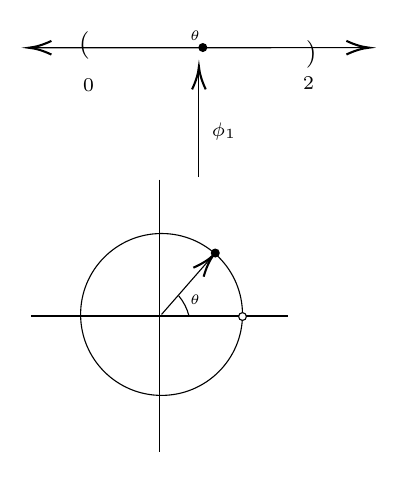
\begin{tikzpicture}[x=0.75pt,y=0.75pt,yscale=-1,xscale=1]
%uncomment if require: \path (0,300); %set diagram left start at 0, and has height of 300

\draw   (121,188.73) -- (245,188.73)(183,123) -- (183,254.47) ;
%Straight Lines [id:da8180273995647878] 
\draw    (122,59.5) -- (282,59.47) ;
\draw [shift={(284,59.47)}, rotate = 179.99] [color={rgb, 255:red, 0; green, 0; blue, 0 }  ][line width=0.75]    (10.93,-3.29) .. controls (6.95,-1.4) and (3.31,-0.3) .. (0,0) .. controls (3.31,0.3) and (6.95,1.4) .. (10.93,3.29)   ;
\draw [shift={(120,59.5)}, rotate = 359.99] [color={rgb, 255:red, 0; green, 0; blue, 0 }  ][line width=0.75]    (10.93,-3.29) .. controls (6.95,-1.4) and (3.31,-0.3) .. (0,0) .. controls (3.31,0.3) and (6.95,1.4) .. (10.93,3.29)   ;
%Shape: Circle [id:dp5128133772288312] 
\draw   (145,188) .. controls (145,166.46) and (162.46,149) .. (184,149) .. controls (205.54,149) and (223,166.46) .. (223,188) .. controls (223,209.54) and (205.54,227) .. (184,227) .. controls (162.46,227) and (145,209.54) .. (145,188) -- cycle ;
%Shape: Circle [id:dp8810895316002555] 
\draw  [fill={rgb, 255:red, 255; green, 255; blue, 255 }  ,fill opacity=1 ] (221.12,189) .. controls (221.12,187.96) and (221.96,187.12) .. (223,187.12) .. controls (224.04,187.12) and (224.88,187.96) .. (224.88,189) .. controls (224.88,190.04) and (224.04,190.88) .. (223,190.88) .. controls (221.96,190.88) and (221.12,190.04) .. (221.12,189) -- cycle ;
%Straight Lines [id:da9436577937186711] 
\draw    (184,188) -- (207.68,160.91) ;
\draw [shift={(209,159.4)}, rotate = 131.16] [color={rgb, 255:red, 0; green, 0; blue, 0 }  ][line width=0.75]    (10.93,-3.29) .. controls (6.95,-1.4) and (3.31,-0.3) .. (0,0) .. controls (3.31,0.3) and (6.95,1.4) .. (10.93,3.29)   ;
%Shape: Arc [id:dp6136432634457998] 
\draw  [draw opacity=0] (192.32,179.07) .. controls (194.56,181.78) and (196.24,184.99) .. (197.17,188.52) -- (174.15,194.94) -- cycle ; \draw   (192.32,179.07) .. controls (194.56,181.78) and (196.24,184.99) .. (197.17,188.52) ;  
%Straight Lines [id:da3473098561653878] 
\draw    (202,121.87) -- (202,70.62) ;
\draw [shift={(202,68.62)}, rotate = 90] [color={rgb, 255:red, 0; green, 0; blue, 0 }  ][line width=0.75]    (10.93,-3.29) .. controls (6.95,-1.4) and (3.31,-0.3) .. (0,0) .. controls (3.31,0.3) and (6.95,1.4) .. (10.93,3.29)   ;
%Shape: Circle [id:dp05894903245242711] 
\draw  [fill={rgb, 255:red, 0; green, 0; blue, 0 }  ,fill opacity=1 ] (208,158.4) .. controls (208,157.36) and (208.84,156.52) .. (209.88,156.52) .. controls (210.92,156.52) and (211.77,157.36) .. (211.77,158.4) .. controls (211.77,159.44) and (210.92,160.28) .. (209.88,160.28) .. controls (208.84,160.28) and (208,159.44) .. (208,158.4) -- cycle ;
%Shape: Circle [id:dp0797933236440207] 
\draw  [fill={rgb, 255:red, 0; green, 0; blue, 0 }  ,fill opacity=1 ] (202,59.4) .. controls (202,58.36) and (202.84,57.52) .. (203.88,57.52) .. controls (204.92,57.52) and (205.77,58.36) .. (205.77,59.4) .. controls (205.77,60.44) and (204.92,61.28) .. (203.88,61.28) .. controls (202.84,61.28) and (202,60.44) .. (202,59.4) -- cycle ;

% Text Node
\draw (196.5,177.1) node [anchor=north west][inner sep=0.75pt]  [font=\tiny]  {$\theta $};
% Text Node

% Text Node
\draw (142.88,50.5) node [anchor=north west][inner sep=0.75pt]  [rotate=-359.08]  {$($};
% Text Node
\draw (259.98,70.62) node [anchor=north west][inner sep=0.75pt]  [rotate=-180.17]  {$($};
% Text Node
\draw (144.88,73.5) node [anchor=north west][inner sep=0.75pt]  [font=\scriptsize,rotate=-359.08]  {$0$};
% Text Node
\draw (250.88,72.5) node [anchor=north west][inner sep=0.75pt]  [font=\scriptsize,rotate=-359.08]  {$2\uppi $};
% Text Node
\draw (196.5,50.1) node [anchor=north west][inner sep=0.75pt]  [font=\tiny]  {$\theta $};
% Text Node
\draw (206.88,94.5) node [anchor=north west][inner sep=0.75pt]  [font=\scriptsize,rotate=-359.08]  {$\phi _{1}$};


\end{tikzpicture}

    \caption{Here the point $(1,0)$ is removed and $\phi_1$ maps the rest of the circle to the interval $(0,2\pi)$.}
    \label{fig:circchart1}
  \end{subfigure}
  \hfill
  \begin{subfigure}[b]{0.45\textwidth}
    \centering
    

\tikzset{every picture/.style={line width=0.75pt}} %set default line width to 0.75pt        

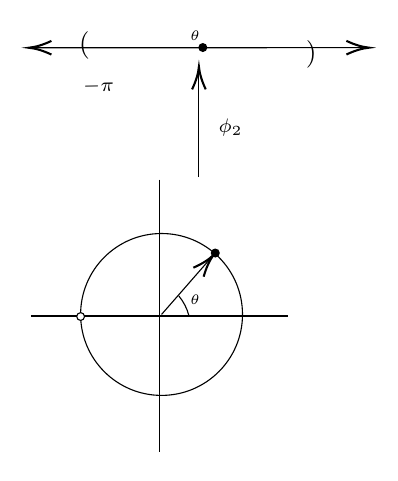
\begin{tikzpicture}[x=0.75pt,y=0.75pt,yscale=-1,xscale=1]
%uncomment if require: \path (0,300); %set diagram left start at 0, and has height of 300

\draw   (258,177.73) -- (382,177.73)(320,112) -- (320,243.47) ;
%Straight Lines [id:da1268514518445265] 
\draw    (259,48.5) -- (419,48.47) ;
\draw [shift={(421,48.47)}, rotate = 179.99] [color={rgb, 255:red, 0; green, 0; blue, 0 }  ][line width=0.75]    (10.93,-3.29) .. controls (6.95,-1.4) and (3.31,-0.3) .. (0,0) .. controls (3.31,0.3) and (6.95,1.4) .. (10.93,3.29)   ;
\draw [shift={(257,48.5)}, rotate = 359.99] [color={rgb, 255:red, 0; green, 0; blue, 0 }  ][line width=0.75]    (10.93,-3.29) .. controls (6.95,-1.4) and (3.31,-0.3) .. (0,0) .. controls (3.31,0.3) and (6.95,1.4) .. (10.93,3.29)   ;
%Shape: Circle [id:dp7024113415149893] 
\draw   (282,177) .. controls (282,155.46) and (299.46,138) .. (321,138) .. controls (342.54,138) and (360,155.46) .. (360,177) .. controls (360,198.54) and (342.54,216) .. (321,216) .. controls (299.46,216) and (282,198.54) .. (282,177) -- cycle ;
%Shape: Circle [id:dp9335574434248441] 
\draw  [fill={rgb, 255:red, 255; green, 255; blue, 255 }  ,fill opacity=1 ] (280.12,178) .. controls (280.12,176.96) and (280.96,176.12) .. (282,176.12) .. controls (283.04,176.12) and (283.88,176.96) .. (283.88,178) .. controls (283.88,179.04) and (283.04,179.88) .. (282,179.88) .. controls (280.96,179.88) and (280.12,179.04) .. (280.12,178) -- cycle ;
%Straight Lines [id:da8252578804556748] 
\draw    (321,177) -- (344.68,149.91) ;
\draw [shift={(346,148.4)}, rotate = 131.16] [color={rgb, 255:red, 0; green, 0; blue, 0 }  ][line width=0.75]    (10.93,-3.29) .. controls (6.95,-1.4) and (3.31,-0.3) .. (0,0) .. controls (3.31,0.3) and (6.95,1.4) .. (10.93,3.29)   ;
%Shape: Arc [id:dp3291144774774024] 
\draw  [draw opacity=0] (329.32,168.07) .. controls (331.56,170.78) and (333.24,173.99) .. (334.17,177.52) -- (311.15,183.94) -- cycle ; \draw   (329.32,168.07) .. controls (331.56,170.78) and (333.24,173.99) .. (334.17,177.52) ;  
%Straight Lines [id:da3615704984807794] 
\draw    (339,110.87) -- (339,59.62) ;
\draw [shift={(339,57.62)}, rotate = 90] [color={rgb, 255:red, 0; green, 0; blue, 0 }  ][line width=0.75]    (10.93,-3.29) .. controls (6.95,-1.4) and (3.31,-0.3) .. (0,0) .. controls (3.31,0.3) and (6.95,1.4) .. (10.93,3.29)   ;
%Shape: Circle [id:dp19768643904648886] 
\draw  [fill={rgb, 255:red, 0; green, 0; blue, 0 }  ,fill opacity=1 ] (345,147.4) .. controls (345,146.36) and (345.84,145.52) .. (346.88,145.52) .. controls (347.92,145.52) and (348.77,146.36) .. (348.77,147.4) .. controls (348.77,148.44) and (347.92,149.28) .. (346.88,149.28) .. controls (345.84,149.28) and (345,148.44) .. (345,147.4) -- cycle ;
%Shape: Circle [id:dp2589693685269747] 
\draw  [fill={rgb, 255:red, 0; green, 0; blue, 0 }  ,fill opacity=1 ] (339,48.4) .. controls (339,47.36) and (339.84,46.52) .. (340.88,46.52) .. controls (341.92,46.52) and (342.77,47.36) .. (342.77,48.4) .. controls (342.77,49.44) and (341.92,50.28) .. (340.88,50.28) .. controls (339.84,50.28) and (339,49.44) .. (339,48.4) -- cycle ;

% Text Node
\draw (333.5,166.1) node [anchor=north west][inner sep=0.75pt]  [font=\tiny]  {$\theta $};
% Text Node

% Text Node
\draw (279.88,39.5) node [anchor=north west][inner sep=0.75pt]  [rotate=-359.08]  {$($};
% Text Node
\draw (396.98,59.62) node [anchor=north west][inner sep=0.75pt]  [rotate=-180.17]  {$($};
% Text Node
\draw (281.88,62.5) node [anchor=north west][inner sep=0.75pt]  [font=\scriptsize,rotate=-359.08]  {$-\pi $};
% Text Node
\draw (387.88,61.5) node [anchor=north west][inner sep=0.75pt]  [font=\scriptsize,rotate=-359.08]  {$\uppi $};
% Text Node
\draw (333.5,39.1) node [anchor=north west][inner sep=0.75pt]  [font=\tiny]  {$\theta $};
% Text Node
\draw (347.05,81.61) node [anchor=north west][inner sep=0.75pt]  [font=\scriptsize,rotate=-359.08]  {$\phi _{2}$};


\end{tikzpicture}

    \caption{Here the point $(-1,0)$ is removed and $\phi_2$ maps the rest of the circle to the interval $(-\pi,\pi)$.}
    \label{fig:circchart2}
  \end{subfigure}
  \caption{$\phi_1$ and $\phi_2$ are invertiable and continuous (easily seen).  The two charts intersect in the upper and lower semicircles (as the antipodal points are removed). The transition function is given by:
  \(\phi_1 \circ \phi_2^{-1}(\theta) = \begin{cases}   \theta  & \text{if } \theta\in (0, \pi) \\  \theta+2\pi & \text{if } \theta \in (-\pi, 0) \end{cases}\)which is \textit{smooth} on each of the semicircles as required. Thus this is a valid chart for the circle.}  
  
\end{figure}
\noindent
The same circle can be described by another chart using the stereographic projection, resulting in the \textbf{Mercator Atlas}. \textcolor{red}{show this maybe}..
Similarly we can prove that the $n$-dimensional sphere is a manifold. 
\subsubsection{Differentiable Maps}
\subsection{Tangent Spaces}
\subsection{Differential Forms}
% \textit{Definition.} Suppose $C\subset \mathbb{R}^2$ be a curve and let $p\in C$ is a point. The tangent space to $C$ at $p$ is the set of all vectors tangent to $C$ at $p$ and is denoted by $T_pC$. 
\end{document}